% Options for packages loaded elsewhere
\PassOptionsToPackage{unicode}{hyperref}
\PassOptionsToPackage{hyphens}{url}
%
\documentclass[
]{article}
\usepackage{amsmath,amssymb}
\usepackage{lmodern}
\usepackage{iftex}
\ifPDFTeX
  \usepackage[T1]{fontenc}
  \usepackage[utf8]{inputenc}
  \usepackage{textcomp} % provide euro and other symbols
\else % if luatex or xetex
  \usepackage{unicode-math}
  \defaultfontfeatures{Scale=MatchLowercase}
  \defaultfontfeatures[\rmfamily]{Ligatures=TeX,Scale=1}
\fi
% Use upquote if available, for straight quotes in verbatim environments
\IfFileExists{upquote.sty}{\usepackage{upquote}}{}
\IfFileExists{microtype.sty}{% use microtype if available
  \usepackage[]{microtype}
  \UseMicrotypeSet[protrusion]{basicmath} % disable protrusion for tt fonts
}{}
\makeatletter
\@ifundefined{KOMAClassName}{% if non-KOMA class
  \IfFileExists{parskip.sty}{%
    \usepackage{parskip}
  }{% else
    \setlength{\parindent}{0pt}
    \setlength{\parskip}{6pt plus 2pt minus 1pt}}
}{% if KOMA class
  \KOMAoptions{parskip=half}}
\makeatother
\usepackage{xcolor}
\usepackage[margin=1in]{geometry}
\usepackage{color}
\usepackage{fancyvrb}
\newcommand{\VerbBar}{|}
\newcommand{\VERB}{\Verb[commandchars=\\\{\}]}
\DefineVerbatimEnvironment{Highlighting}{Verbatim}{commandchars=\\\{\}}
% Add ',fontsize=\small' for more characters per line
\usepackage{framed}
\definecolor{shadecolor}{RGB}{248,248,248}
\newenvironment{Shaded}{\begin{snugshade}}{\end{snugshade}}
\newcommand{\AlertTok}[1]{\textcolor[rgb]{0.94,0.16,0.16}{#1}}
\newcommand{\AnnotationTok}[1]{\textcolor[rgb]{0.56,0.35,0.01}{\textbf{\textit{#1}}}}
\newcommand{\AttributeTok}[1]{\textcolor[rgb]{0.77,0.63,0.00}{#1}}
\newcommand{\BaseNTok}[1]{\textcolor[rgb]{0.00,0.00,0.81}{#1}}
\newcommand{\BuiltInTok}[1]{#1}
\newcommand{\CharTok}[1]{\textcolor[rgb]{0.31,0.60,0.02}{#1}}
\newcommand{\CommentTok}[1]{\textcolor[rgb]{0.56,0.35,0.01}{\textit{#1}}}
\newcommand{\CommentVarTok}[1]{\textcolor[rgb]{0.56,0.35,0.01}{\textbf{\textit{#1}}}}
\newcommand{\ConstantTok}[1]{\textcolor[rgb]{0.00,0.00,0.00}{#1}}
\newcommand{\ControlFlowTok}[1]{\textcolor[rgb]{0.13,0.29,0.53}{\textbf{#1}}}
\newcommand{\DataTypeTok}[1]{\textcolor[rgb]{0.13,0.29,0.53}{#1}}
\newcommand{\DecValTok}[1]{\textcolor[rgb]{0.00,0.00,0.81}{#1}}
\newcommand{\DocumentationTok}[1]{\textcolor[rgb]{0.56,0.35,0.01}{\textbf{\textit{#1}}}}
\newcommand{\ErrorTok}[1]{\textcolor[rgb]{0.64,0.00,0.00}{\textbf{#1}}}
\newcommand{\ExtensionTok}[1]{#1}
\newcommand{\FloatTok}[1]{\textcolor[rgb]{0.00,0.00,0.81}{#1}}
\newcommand{\FunctionTok}[1]{\textcolor[rgb]{0.00,0.00,0.00}{#1}}
\newcommand{\ImportTok}[1]{#1}
\newcommand{\InformationTok}[1]{\textcolor[rgb]{0.56,0.35,0.01}{\textbf{\textit{#1}}}}
\newcommand{\KeywordTok}[1]{\textcolor[rgb]{0.13,0.29,0.53}{\textbf{#1}}}
\newcommand{\NormalTok}[1]{#1}
\newcommand{\OperatorTok}[1]{\textcolor[rgb]{0.81,0.36,0.00}{\textbf{#1}}}
\newcommand{\OtherTok}[1]{\textcolor[rgb]{0.56,0.35,0.01}{#1}}
\newcommand{\PreprocessorTok}[1]{\textcolor[rgb]{0.56,0.35,0.01}{\textit{#1}}}
\newcommand{\RegionMarkerTok}[1]{#1}
\newcommand{\SpecialCharTok}[1]{\textcolor[rgb]{0.00,0.00,0.00}{#1}}
\newcommand{\SpecialStringTok}[1]{\textcolor[rgb]{0.31,0.60,0.02}{#1}}
\newcommand{\StringTok}[1]{\textcolor[rgb]{0.31,0.60,0.02}{#1}}
\newcommand{\VariableTok}[1]{\textcolor[rgb]{0.00,0.00,0.00}{#1}}
\newcommand{\VerbatimStringTok}[1]{\textcolor[rgb]{0.31,0.60,0.02}{#1}}
\newcommand{\WarningTok}[1]{\textcolor[rgb]{0.56,0.35,0.01}{\textbf{\textit{#1}}}}
\usepackage{longtable,booktabs,array}
\usepackage{calc} % for calculating minipage widths
% Correct order of tables after \paragraph or \subparagraph
\usepackage{etoolbox}
\makeatletter
\patchcmd\longtable{\par}{\if@noskipsec\mbox{}\fi\par}{}{}
\makeatother
% Allow footnotes in longtable head/foot
\IfFileExists{footnotehyper.sty}{\usepackage{footnotehyper}}{\usepackage{footnote}}
\makesavenoteenv{longtable}
\usepackage{graphicx}
\makeatletter
\def\maxwidth{\ifdim\Gin@nat@width>\linewidth\linewidth\else\Gin@nat@width\fi}
\def\maxheight{\ifdim\Gin@nat@height>\textheight\textheight\else\Gin@nat@height\fi}
\makeatother
% Scale images if necessary, so that they will not overflow the page
% margins by default, and it is still possible to overwrite the defaults
% using explicit options in \includegraphics[width, height, ...]{}
\setkeys{Gin}{width=\maxwidth,height=\maxheight,keepaspectratio}
% Set default figure placement to htbp
\makeatletter
\def\fps@figure{htbp}
\makeatother
\setlength{\emergencystretch}{3em} % prevent overfull lines
\providecommand{\tightlist}{%
  \setlength{\itemsep}{0pt}\setlength{\parskip}{0pt}}
\setcounter{secnumdepth}{-\maxdimen} % remove section numbering
\ifLuaTeX
  \usepackage{selnolig}  % disable illegal ligatures
\fi
\IfFileExists{bookmark.sty}{\usepackage{bookmark}}{\usepackage{hyperref}}
\IfFileExists{xurl.sty}{\usepackage{xurl}}{} % add URL line breaks if available
\urlstyle{same} % disable monospaced font for URLs
\hypersetup{
  pdftitle={Entrega PG 1 - Gestor de Motor de busqueda para elaborar recomendaciones sobre las preferencias de la Ropa de moda de la India},
  hidelinks,
  pdfcreator={LaTeX via pandoc}}

\title{Entrega PG 1 - Gestor de Motor de busqueda para elaborar
recomendaciones sobre las preferencias de la Ropa de moda de la India}
\author{}
\date{\vspace{-2.5em}30 Agosto, 2023}

\begin{document}
\maketitle

{
\setcounter{tocdepth}{5}
\tableofcontents
}
\begin{quote}
\hypertarget{introducciuxf3n}{%
\section{\texorpdfstring{\textbf{Introducción}}{Introducción}}\label{introducciuxf3n}}
\end{quote}

La moda es una industria global en constante evolución y uno de los
mayores impulsores del comercio internacional. Los consumidores buscan
constantemente nuevas tendencias y estilos únicos, lo que hace que la
industria de la moda sea altamente competitiva. Para ayudar a los
minoristas a mantenerse al día con las últimas tendencias y preferencias
de los consumidores, se están desarrollando nuevas herramientas de
análisis de datos y motores de búsqueda para la moda.

\begin{quote}
\hypertarget{relevancia-y-justificaciuxf3n}{%
\subsubsection{\texorpdfstring{\textbf{\emph{Relevancia y
Justificación:}}}{Relevancia y Justificación:}}\label{relevancia-y-justificaciuxf3n}}
\end{quote}

En este contexto, el desarrollo de un gestor de motor de búsqueda para
la elaboración de recomendaciones sobre las preferencias de la ropa de
moda en la India se vuelve crucial para mejorar la capacidad de las
empresas de este sector, ya que permite ofrecer productos más acordes a
las necesidades y gustos de los consumidores. Además, este tipo de
herramientas tecnológicas permiten recopilar grandes cantidades de datos
sobre las preferencias de los consumidores de manera eficiente, lo que
es vital para mejorar la eficacia y eficiencia de la toma de decisiones
empresariales.

\begin{quote}
\hypertarget{objetivos}{%
\section{\texorpdfstring{\textbf{Objetivos:}}{Objetivos:}}\label{objetivos}}

\hypertarget{objetivo-principal}{%
\subsubsection{\texorpdfstring{\textbf{Objetivo
Principal:}}{Objetivo Principal:}}\label{objetivo-principal}}
\end{quote}

Nuestro objetivo de este trabajo es presentar un gestor de motor de
búsqueda para elaborar recomendaciones sobre las preferencias de la ropa
de moda en la India. Para ello, se analizará una base de datos,
\href{BaseDatos}{MYNTRA}, que incluye información sobre los \emph{gustos
y preferencias de los consumidores} en cuanto a diferentes tipos de
prendas y estilos de moda.

\begin{quote}
\hypertarget{objetivos-secundarios}{%
\subsubsection{\texorpdfstring{\textbf{\emph{Objetivos
Secundarios}}}{Objetivos Secundarios}}\label{objetivos-secundarios}}
\end{quote}

A partir de esta información, se desarrollará un modelo de recomendación
que permita a las empresas del sector ofrecer productos más acordes a
las necesidades y gustos de los consumidores, contribuyendo así a
mejorar su competitividad y su capacidad de satisfacer las demandas del
mercado.

\begin{itemize}
\tightlist
\item
  Identificar los productos más caros
\item
  Identificar los colores más repetidos que llevan el aumento de precio
\item
  Identificar que productos que prefiere la población, su precio, color
  y para que géneros
\item
  Analizar qué productos en el mercado de la India son más caros y para
  qué género
\item
  Identificar los colores preferidos de la población con relación a su
  género
\end{itemize}

\begin{quote}
\hypertarget{datos}{%
\section{\texorpdfstring{\textbf{\emph{Datos}}}{Datos}}\label{datos}}

\hypertarget{recolecciuxf3n-de-datos}{%
\subsubsection{\texorpdfstring{\textbf{\emph{Recolección de
datos}}}{Recolección de datos}}\label{recolecciuxf3n-de-datos}}
\end{quote}

Se ha seleccionado la data de una base de datos de Kaggle con el nombre
\href{BaseDatos}{``Fashion Clothing Products Dataset''} el cual presenta
una población de 10000 valores. La base de datos se origina en
Myntra.com, Myntra es una importante empresa india de comercio
electrónico de moda con sede en Bengaluru, Karnataka, India. La empresa
se fundó en 2007 para vender artículos de regalo personalizados. En mayo
de 2014 , FlipKart adquirió Myntra.com.

Empezaremos cargando nuestra base de datos

\begin{Shaded}
\begin{Highlighting}[]
\FunctionTok{library}\NormalTok{(readr)}
\FunctionTok{library}\NormalTok{(dplyr)}
\FunctionTok{library}\NormalTok{(modeest)}
\FunctionTok{library}\NormalTok{(ggplot2)}
\FunctionTok{library}\NormalTok{(plotrix)}

\NormalTok{dataframe}\OtherTok{\textless{}{-}}\FunctionTok{read\_csv}\NormalTok{(}\StringTok{"myntra\_products\_catalog.csv"}\NormalTok{)}
\NormalTok{dataframe}
\end{Highlighting}
\end{Shaded}

\begin{verbatim}
## # A tibble: 12,491 x 8
##    ProductID ProductName ProductBrand Gender `Price (INR)` NumImages Description
##        <dbl> <chr>       <chr>        <chr>          <dbl>     <dbl> <chr>      
##  1  10017413 DKNY Unise~ DKNY         Unisex         11745         7 Black and ~
##  2  10016283 EthnoVogue~ EthnoVogue   Women           5810         7 Beige & Gr~
##  3  10009781 SPYKAR Wom~ SPYKAR       Women            899         7 Pink colou~
##  4  10015921 Raymond Me~ Raymond      Men             5599         5 Blue self-~
##  5  10017833 Parx Men B~ Parx         Men              759         5 Brown and ~
##  6  10014361 SHOWOFF Me~ SHOWOFF      Men              791         5 Brown soli~
##  7  10017869 Parx Men B~ Parx         Men              719         5 Blue check~
##  8  10009695 SPYKAR Wom~ SPYKAR       Women            899         7 Burgundy c~
##  9  10000571 Parx Men B~ Parx         Men              664         5 Brown soli~
## 10  10017421 DKNY Unise~ DKNY         Unisex         17360         5 Black soli~
## # i 12,481 more rows
## # i 1 more variable: PrimaryColor <chr>
\end{verbatim}

\begin{quote}
\hypertarget{poblaciuxf3n-objetivo}{%
\subsubsection{\texorpdfstring{\textbf{\emph{Población
Objetivo}}}{Población Objetivo}}\label{poblaciuxf3n-objetivo}}
\end{quote}

Seleccionaremos una muestra de 1000 variables para poder cumplir
nuestros objetivos y poder responder de manera adecuada cada pregunta
usando los análisis y limpieza de los datos que hemos aprendido a lo
largo de este curso.

A continuación seleccionaremos nuestra muestra

\begin{Shaded}
\begin{Highlighting}[]
\NormalTok{dataMuestra}\OtherTok{\textless{}{-}}\NormalTok{dataframe[}\DecValTok{1}\SpecialCharTok{:}\DecValTok{1000}\NormalTok{,]}
\NormalTok{dataMuestra}
\end{Highlighting}
\end{Shaded}

\begin{verbatim}
## # A tibble: 1,000 x 8
##    ProductID ProductName ProductBrand Gender `Price (INR)` NumImages Description
##        <dbl> <chr>       <chr>        <chr>          <dbl>     <dbl> <chr>      
##  1  10017413 DKNY Unise~ DKNY         Unisex         11745         7 Black and ~
##  2  10016283 EthnoVogue~ EthnoVogue   Women           5810         7 Beige & Gr~
##  3  10009781 SPYKAR Wom~ SPYKAR       Women            899         7 Pink colou~
##  4  10015921 Raymond Me~ Raymond      Men             5599         5 Blue self-~
##  5  10017833 Parx Men B~ Parx         Men              759         5 Brown and ~
##  6  10014361 SHOWOFF Me~ SHOWOFF      Men              791         5 Brown soli~
##  7  10017869 Parx Men B~ Parx         Men              719         5 Blue check~
##  8  10009695 SPYKAR Wom~ SPYKAR       Women            899         7 Burgundy c~
##  9  10000571 Parx Men B~ Parx         Men              664         5 Brown soli~
## 10  10017421 DKNY Unise~ DKNY         Unisex         17360         5 Black soli~
## # i 990 more rows
## # i 1 more variable: PrimaryColor <chr>
\end{verbatim}

y continuaremos con nuestro estudio en base a esta

\begin{quote}
\hypertarget{variables-de-estudio-iniciales}{%
\section{\texorpdfstring{\textbf{\emph{Variables de estudio
iniciales}}}{Variables de estudio iniciales}}\label{variables-de-estudio-iniciales}}
\end{quote}

Para la base de datos presentamos las siguientes variables:

\begin{longtable}[]{@{}
  >{\centering\arraybackslash}p{(\columnwidth - 4\tabcolsep) * \real{0.3667}}
  >{\centering\arraybackslash}p{(\columnwidth - 4\tabcolsep) * \real{0.3667}}
  >{\centering\arraybackslash}p{(\columnwidth - 4\tabcolsep) * \real{0.2667}}@{}}
\toprule()
\begin{minipage}[b]{\linewidth}\centering
\textbf{Nombre de variable}
\end{minipage} & \begin{minipage}[b]{\linewidth}\centering
\textbf{Tipo de variable}
\end{minipage} & \begin{minipage}[b]{\linewidth}\centering
\textbf{Descripción}
\end{minipage} \\
\midrule()
\endhead
\textbf{ProductoId} & \textbf{\emph{cualitativa}} & Es nuestra llave
primaria para cada producto, única en toda la base de datos \\
\textbf{NombreProducto} & \textbf{\emph{cualitativa}} & El nombre del
producto \\
\textbf{MarcaProducto} & \textbf{\emph{cualitativa}} & La marca que
fabrica el producto \\
\textbf{Género} & \textbf{\emph{cualitativa}} & El género el cual esta
destinado para el producto \\
\textbf{PrecioUSD} & \textbf{\emph{cuantitativa}} & El precio en
Rupias(INR) convertido a dolares estadounidenses(USD) \\
\textbf{NumImagenes} & \textbf{\emph{cuantitativa}} & Cantidad de
imágenes que hay para el producto \\
\textbf{Descripción} & \textbf{\emph{cualitativa}} & Una pequeña
descripción sobre el producto \\
\textbf{ColorPrimario} & \textbf{\emph{cualitativa}} & Color del
producto \\
\bottomrule()
\end{longtable}

Actualizamos el nombre de nuestras columnas para una mejor visualización
de nuestro estudio.

\begin{Shaded}
\begin{Highlighting}[]
\FunctionTok{colnames}\NormalTok{(dataMuestra)}
\end{Highlighting}
\end{Shaded}

\begin{verbatim}
## [1] "ProductID"    "ProductName"  "ProductBrand" "Gender"       "Price (INR)" 
## [6] "NumImages"    "Description"  "PrimaryColor"
\end{verbatim}

\begin{Shaded}
\begin{Highlighting}[]
\FunctionTok{colnames}\NormalTok{(dataMuestra)}\OtherTok{\textless{}{-}}\FunctionTok{c}\NormalTok{(}\StringTok{"ProductoId"}\NormalTok{,}\StringTok{"NombreProducto"}\NormalTok{,}\StringTok{"MarcaProducto"}\NormalTok{,}\StringTok{"Genero"}\NormalTok{,}\StringTok{"PrecioUSD"}\NormalTok{,}\StringTok{"NumImagenes"}\NormalTok{,}\StringTok{"Descripción"}\NormalTok{,}\StringTok{"ColorPrimario"}\NormalTok{)}
\end{Highlighting}
\end{Shaded}

\textbf{\emph{Ahora nuestras columnas se llamaran}}

\begin{Shaded}
\begin{Highlighting}[]
\FunctionTok{colnames}\NormalTok{(dataMuestra)}
\end{Highlighting}
\end{Shaded}

\begin{verbatim}
## [1] "ProductoId"     "NombreProducto" "MarcaProducto"  "Genero"        
## [5] "PrecioUSD"      "NumImagenes"    "Descripción"    "ColorPrimario"
\end{verbatim}

\textbf{\emph{Control de los Na en las variables}}

\begin{Shaded}
\begin{Highlighting}[]
\FunctionTok{any}\NormalTok{(}\FunctionTok{is.na}\NormalTok{(dataMuestra}\SpecialCharTok{$}\NormalTok{ProductoId))}
\end{Highlighting}
\end{Shaded}

\begin{verbatim}
## [1] FALSE
\end{verbatim}

\begin{Shaded}
\begin{Highlighting}[]
\FunctionTok{any}\NormalTok{(}\FunctionTok{is.na}\NormalTok{(dataMuestra}\SpecialCharTok{$}\NormalTok{NombreProducto))}
\end{Highlighting}
\end{Shaded}

\begin{verbatim}
## [1] FALSE
\end{verbatim}

\begin{Shaded}
\begin{Highlighting}[]
\FunctionTok{any}\NormalTok{(}\FunctionTok{is.na}\NormalTok{(dataMuestra}\SpecialCharTok{$}\NormalTok{MarcaProducto))}
\end{Highlighting}
\end{Shaded}

\begin{verbatim}
## [1] FALSE
\end{verbatim}

\begin{Shaded}
\begin{Highlighting}[]
\FunctionTok{any}\NormalTok{(}\FunctionTok{is.na}\NormalTok{(dataMuestra}\SpecialCharTok{$}\NormalTok{Genero))}
\end{Highlighting}
\end{Shaded}

\begin{verbatim}
## [1] FALSE
\end{verbatim}

\begin{Shaded}
\begin{Highlighting}[]
\FunctionTok{any}\NormalTok{(}\FunctionTok{is.na}\NormalTok{(dataMuestra}\SpecialCharTok{$}\NormalTok{PrecioUSD))}
\end{Highlighting}
\end{Shaded}

\begin{verbatim}
## [1] FALSE
\end{verbatim}

\begin{Shaded}
\begin{Highlighting}[]
\FunctionTok{any}\NormalTok{(}\FunctionTok{is.na}\NormalTok{(dataMuestra}\SpecialCharTok{$}\NormalTok{NumImagenes))}
\end{Highlighting}
\end{Shaded}

\begin{verbatim}
## [1] FALSE
\end{verbatim}

\begin{Shaded}
\begin{Highlighting}[]
\FunctionTok{any}\NormalTok{(}\FunctionTok{is.na}\NormalTok{(dataMuestra}\SpecialCharTok{$}\NormalTok{Descripción))}
\end{Highlighting}
\end{Shaded}

\begin{verbatim}
## [1] FALSE
\end{verbatim}

\begin{Shaded}
\begin{Highlighting}[]
\FunctionTok{any}\NormalTok{(}\FunctionTok{is.na}\NormalTok{(dataMuestra}\SpecialCharTok{$}\NormalTok{ColorPrimario))}
\end{Highlighting}
\end{Shaded}

\begin{verbatim}
## [1] TRUE
\end{verbatim}

Detectamos que color primario cuenta con valores Na entonces procedemos
a corregirlo

\begin{Shaded}
\begin{Highlighting}[]
\NormalTok{dataMuestra}\SpecialCharTok{$}\NormalTok{ColorPrimario[}\FunctionTok{is.na}\NormalTok{(dataMuestra}\SpecialCharTok{$}\NormalTok{ColorPrimario)]}\OtherTok{\textless{}{-}}\StringTok{"No color"}
\FunctionTok{any}\NormalTok{(}\FunctionTok{is.na}\NormalTok{(dataMuestra}\SpecialCharTok{$}\NormalTok{ColorPrimario))}
\end{Highlighting}
\end{Shaded}

\begin{verbatim}
## [1] FALSE
\end{verbatim}

Convertimos la rupia del Precio del producto a dolares estadounidenses

\begin{Shaded}
\begin{Highlighting}[]
\NormalTok{dataMuestra}\SpecialCharTok{$}\NormalTok{PrecioUSD}\OtherTok{\textless{}{-}}\NormalTok{dataMuestra}\SpecialCharTok{$}\NormalTok{PrecioUSD}\SpecialCharTok{*}\FloatTok{0.012}
\NormalTok{dataMuestra}\SpecialCharTok{$}\NormalTok{PrecioUSD[}\DecValTok{1}\SpecialCharTok{:}\DecValTok{10}\NormalTok{]}
\end{Highlighting}
\end{Shaded}

\begin{verbatim}
##  [1] 140.940  69.720  10.788  67.188   9.108   9.492   8.628  10.788   7.968
## [10] 208.320
\end{verbatim}

\begin{quote}
\hypertarget{anuxe1lisis-descriptivo}{%
\section{\texorpdfstring{\textbf{\emph{Análisis
descriptivo}}}{Análisis descriptivo}}\label{anuxe1lisis-descriptivo}}
\end{quote}

\textbf{\emph{La moda de los productos: }}

\begin{Shaded}
\begin{Highlighting}[]
\NormalTok{getmode }\OtherTok{\textless{}{-}} \ControlFlowTok{function}\NormalTok{(mod) \{}
\NormalTok{   uniqv }\OtherTok{\textless{}{-}} \FunctionTok{unique}\NormalTok{(mod)}
\NormalTok{   uniqv[}\FunctionTok{which.max}\NormalTok{(}\FunctionTok{tabulate}\NormalTok{(}\FunctionTok{match}\NormalTok{(mod, uniqv)))]}
\NormalTok{\}}
\NormalTok{modNombreProducto }\OtherTok{\textless{}{-}}\NormalTok{ dataMuestra}\SpecialCharTok{$}\NormalTok{NombreProducto}
\NormalTok{result }\OtherTok{\textless{}{-}} \FunctionTok{getmode}\NormalTok{(modNombreProducto)}
\FunctionTok{print}\NormalTok{(result)}
\end{Highlighting}
\end{Shaded}

\begin{verbatim}
## [1] "Parx Men Blue Slim Fit Checked Casual Shirt"
\end{verbatim}

\begin{Shaded}
\begin{Highlighting}[]
\CommentTok{\#OTRA FORMA}
\FunctionTok{mfv}\NormalTok{(dataMuestra}\SpecialCharTok{$}\NormalTok{NombreProducto,}\AttributeTok{method=}\StringTok{"mlv"}\NormalTok{)}
\end{Highlighting}
\end{Shaded}

\begin{verbatim}
## [1] "Parx Men Blue Slim Fit Checked Casual Shirt"
\end{verbatim}

A partir de esta función, podemos determinar e producto que más se
repite, es decir, el que posee mayor demanda por los consumidores. En
este caso es ``Parx Men Blue Slim Fit Checked Casual Shirt''.

\begin{Shaded}
\begin{Highlighting}[]
\NormalTok{tablaNombreProducto}\OtherTok{\textless{}{-}}\FunctionTok{table}\NormalTok{(modNombreProducto)}

\NormalTok{maxNombreProducto}\OtherTok{\textless{}{-}}\FunctionTok{max}\NormalTok{(tablaNombreProducto)}
\FunctionTok{print}\NormalTok{(maxNombreProducto)}
\end{Highlighting}
\end{Shaded}

\begin{verbatim}
## [1] 16
\end{verbatim}

\begin{Shaded}
\begin{Highlighting}[]
\CommentTok{\# Convertir la tabla en un dataframe}
\NormalTok{tabla\_df }\OtherTok{\textless{}{-}} \FunctionTok{as.data.frame}\NormalTok{(tablaNombreProducto)}
\CommentTok{\# Acceder al conteo}
\NormalTok{conteo }\OtherTok{\textless{}{-}}\NormalTok{ tabla\_df}\SpecialCharTok{$}\NormalTok{Freq}
\CommentTok{\# Definir el valor umbral para cambiar el color de la barra}
\FunctionTok{ggplot}\NormalTok{(tabla\_df,}\FunctionTok{aes}\NormalTok{(}\AttributeTok{x=}\NormalTok{tabla\_df}\SpecialCharTok{$}\NormalTok{modNombreProducto,}\AttributeTok{y=}\NormalTok{tabla\_df}\SpecialCharTok{$}\NormalTok{Freq)) }\SpecialCharTok{+}
  \FunctionTok{geom\_bar}\NormalTok{(}\AttributeTok{stat =} \StringTok{"identity"}\NormalTok{, }\AttributeTok{fill =} \FunctionTok{ifelse}\NormalTok{(conteo }\SpecialCharTok{==}\NormalTok{ maxNombreProducto, }\StringTok{"green"}\NormalTok{, }\StringTok{"blue"}\NormalTok{)) }\SpecialCharTok{+}
  \FunctionTok{labs}\NormalTok{(}\AttributeTok{x =} \StringTok{"Nombre Producto"}\NormalTok{, }\AttributeTok{y =} \StringTok{"Cant. Apariciones"}\NormalTok{) }\SpecialCharTok{+}
  \FunctionTok{ggtitle}\NormalTok{(}\StringTok{"Gráfico de barras {-} NombreProducto"}\NormalTok{) }\SpecialCharTok{+}
  \FunctionTok{theme\_minimal}\NormalTok{()}
\end{Highlighting}
\end{Shaded}

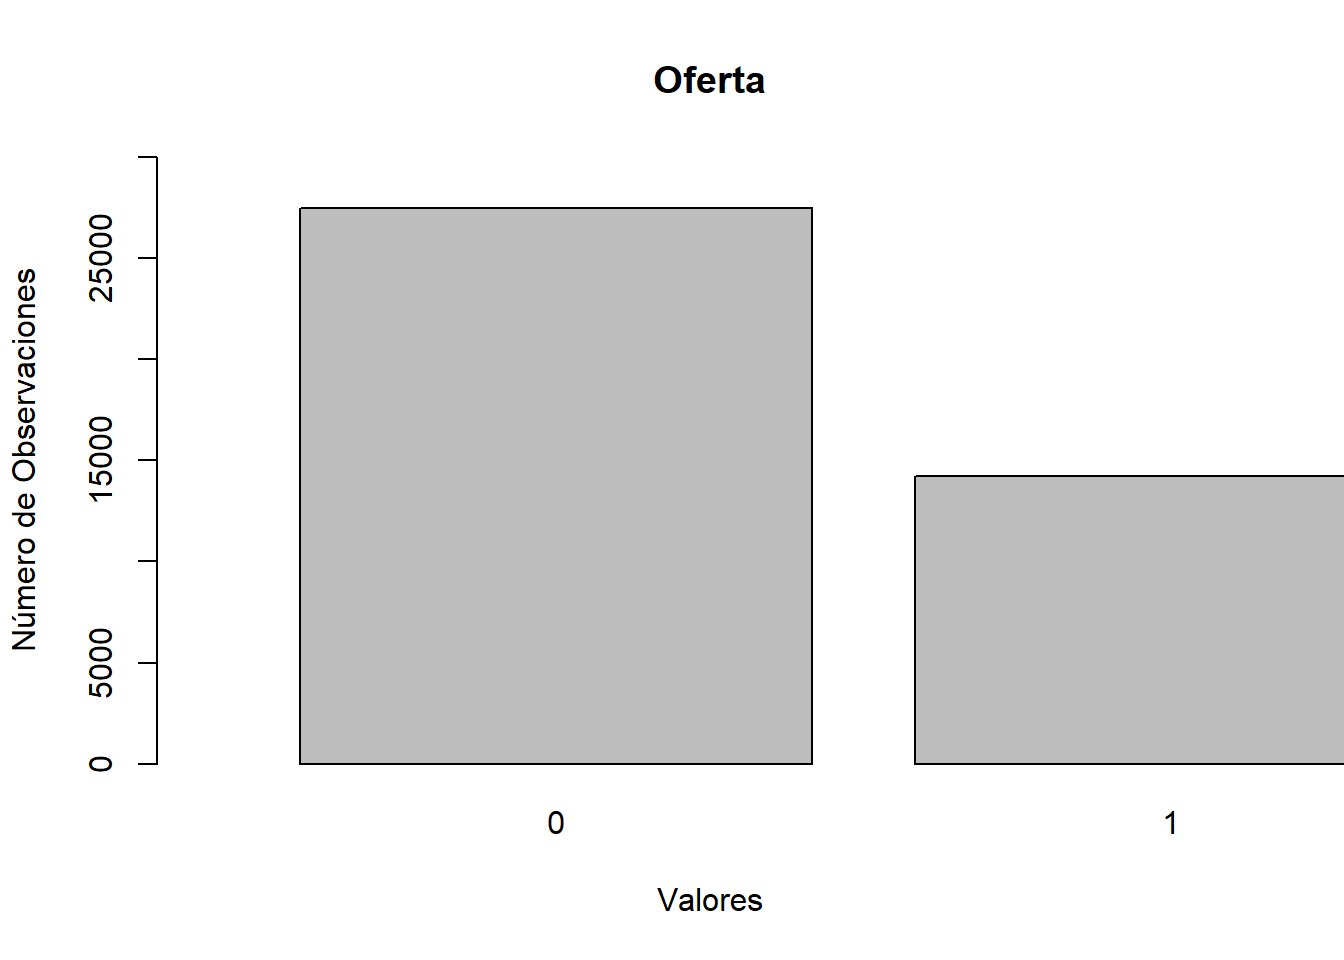
\includegraphics{S3_Informe_files/figure-latex/unnamed-chunk-10-1.pdf}

\begin{Shaded}
\begin{Highlighting}[]
\NormalTok{ProductosPreferidos}\OtherTok{\textless{}{-}}\NormalTok{dataMuestra }\SpecialCharTok{\%\textgreater{}\%}
  \FunctionTok{filter}\NormalTok{(dataMuestra}\SpecialCharTok{$}\NormalTok{NombreProducto}\SpecialCharTok{==}\NormalTok{result)}

\NormalTok{precios}\OtherTok{\textless{}{-}} \FunctionTok{as.data.frame}\NormalTok{(}\FunctionTok{table}\NormalTok{(ProductosPreferidos}\SpecialCharTok{$}\NormalTok{PrecioUSD))}
\NormalTok{colores}\OtherTok{\textless{}{-}}\FunctionTok{as.data.frame}\NormalTok{(}\FunctionTok{table}\NormalTok{(ProductosPreferidos}\SpecialCharTok{$}\NormalTok{ColorPrimario))}
\NormalTok{sexos}\OtherTok{\textless{}{-}}\FunctionTok{as.data.frame}\NormalTok{(}\FunctionTok{table}\NormalTok{(ProductosPreferidos}\SpecialCharTok{$}\NormalTok{Genero))}
\end{Highlighting}
\end{Shaded}

\begin{quote}
\hypertarget{explicaciuxf3n}{%
\subsection{\texorpdfstring{\textbf{\emph{EXPLICACIÓN:}}}{EXPLICACIÓN:}}\label{explicaciuxf3n}}
\end{quote}

Podemos observar en mediante este gráfico de barras que el nombre que
más pedido en MYNTRA es ``Parx Men Blue Slim Fit Checked Casual Shirt''
con un total de 16 veces pedido. Además de que su rango de precios es
entre:

\begin{Shaded}
\begin{Highlighting}[]
\FunctionTok{range}\NormalTok{(}\FunctionTok{as.double}\NormalTok{(}\FunctionTok{as.character}\NormalTok{(precios}\SpecialCharTok{$}\NormalTok{Var1)))}
\end{Highlighting}
\end{Shaded}

\begin{verbatim}
## [1]  8.148 11.268
\end{verbatim}

\begin{Shaded}
\begin{Highlighting}[]
\FunctionTok{print}\NormalTok{(colores}\SpecialCharTok{$}\NormalTok{Var1)}
\end{Highlighting}
\end{Shaded}

\begin{verbatim}
## [1] Blue
## Levels: Blue
\end{verbatim}

\begin{Shaded}
\begin{Highlighting}[]
\FunctionTok{print}\NormalTok{(sexos}\SpecialCharTok{$}\NormalTok{Var1)}
\end{Highlighting}
\end{Shaded}

\begin{verbatim}
## [1] Men
## Levels: Men
\end{verbatim}

Podemos concluir que los hombres, que compran ``Parx Men Blue Slim Fit
Checked Casual Shirt'' a un precio entre 8.148 y 11.268 les gusta el
color azul, además de que tambien es el producto.

\textbf{\emph{La moda de la marca del producto:}}

\begin{Shaded}
\begin{Highlighting}[]
\NormalTok{getmode }\OtherTok{\textless{}{-}} \ControlFlowTok{function}\NormalTok{(mod) \{}
\NormalTok{   uniqv }\OtherTok{\textless{}{-}} \FunctionTok{unique}\NormalTok{(mod)}
\NormalTok{   uniqv[}\FunctionTok{which.max}\NormalTok{(}\FunctionTok{tabulate}\NormalTok{(}\FunctionTok{match}\NormalTok{(mod, uniqv)))]}
\NormalTok{\}}

\NormalTok{mod }\OtherTok{\textless{}{-}}\NormalTok{ dataMuestra}\SpecialCharTok{$}\NormalTok{MarcaProducto}

\NormalTok{result }\OtherTok{\textless{}{-}} \FunctionTok{getmode}\NormalTok{(mod)}
\FunctionTok{print}\NormalTok{(result)}
\end{Highlighting}
\end{Shaded}

\begin{verbatim}
## [1] "Parx"
\end{verbatim}

A partir de esta función, podemos determinar que la marca del producto
que más se repite, es decir, la marca de preferencia por la población
muestrada es ``Parx''.

\begin{Shaded}
\begin{Highlighting}[]
\NormalTok{tablaMarca}\OtherTok{\textless{}{-}}\FunctionTok{table}\NormalTok{(dataMuestra}\SpecialCharTok{$}\NormalTok{MarcaProducto)}

\NormalTok{maxMarca}\OtherTok{\textless{}{-}}\FunctionTok{max}\NormalTok{(}\FunctionTok{table}\NormalTok{(dataMuestra}\SpecialCharTok{$}\NormalTok{MarcaProducto))}
\FunctionTok{print}\NormalTok{(maxMarca)}
\end{Highlighting}
\end{Shaded}

\begin{verbatim}
## [1] 112
\end{verbatim}

\begin{Shaded}
\begin{Highlighting}[]
\CommentTok{\# Convertir la tabla en un dataframe}
\NormalTok{tabla\_df }\OtherTok{\textless{}{-}} \FunctionTok{as.data.frame}\NormalTok{(tablaMarca)}
\CommentTok{\# Acceder al conteo}
\NormalTok{conteo }\OtherTok{\textless{}{-}}\NormalTok{ tabla\_df}\SpecialCharTok{$}\NormalTok{Freq}
\CommentTok{\# Definir el valor umbral para cambiar el color de la barra}
\FunctionTok{ggplot}\NormalTok{(tabla\_df,}\FunctionTok{aes}\NormalTok{(}\AttributeTok{x=}\NormalTok{tabla\_df}\SpecialCharTok{$}\NormalTok{Var1,}\AttributeTok{y=}\NormalTok{tabla\_df}\SpecialCharTok{$}\NormalTok{Freq)) }\SpecialCharTok{+}
  \FunctionTok{geom\_bar}\NormalTok{(}\AttributeTok{stat =} \StringTok{"identity"}\NormalTok{, }\AttributeTok{fill =} \FunctionTok{ifelse}\NormalTok{(conteo }\SpecialCharTok{==}\NormalTok{ maxMarca, }\StringTok{"green"}\NormalTok{, }\StringTok{"blue"}\NormalTok{)) }\SpecialCharTok{+}
  \FunctionTok{labs}\NormalTok{(}\AttributeTok{x =} \StringTok{"Marca Producto"}\NormalTok{, }\AttributeTok{y =} \StringTok{"Cant. Apariciones"}\NormalTok{) }\SpecialCharTok{+}
  \CommentTok{\#ggline(promedioMarca \textasciitilde{}range())}
  \FunctionTok{ggtitle}\NormalTok{(}\StringTok{"Gráfico de barras {-} MarcaProducto"}\NormalTok{) }\SpecialCharTok{+}
  \FunctionTok{theme\_minimal}\NormalTok{()}
\end{Highlighting}
\end{Shaded}

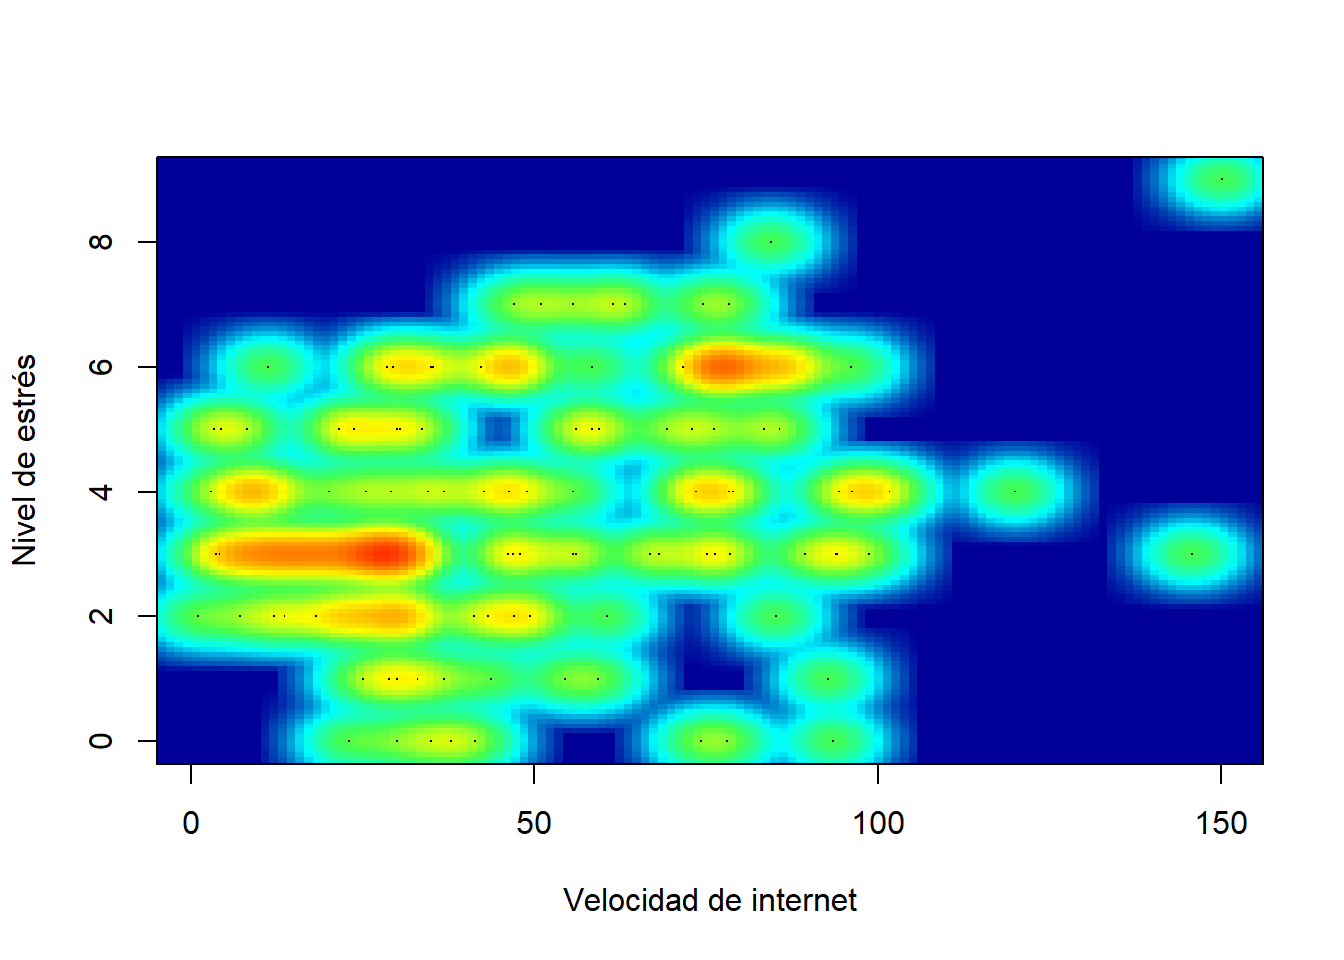
\includegraphics{S3_Informe_files/figure-latex/unnamed-chunk-13-1.pdf}

\begin{Shaded}
\begin{Highlighting}[]
\NormalTok{MarcaPreferida}\OtherTok{\textless{}{-}}\NormalTok{dataMuestra}\SpecialCharTok{\%\textgreater{}\%}
  \FunctionTok{filter}\NormalTok{(dataMuestra}\SpecialCharTok{$}\NormalTok{MarcaProducto}\SpecialCharTok{==}\NormalTok{result)}
\NormalTok{precio}\OtherTok{\textless{}{-}}\FunctionTok{as.data.frame}\NormalTok{(}\FunctionTok{table}\NormalTok{(MarcaPreferida}\SpecialCharTok{$}\NormalTok{PrecioUSD))}
\NormalTok{color}\OtherTok{\textless{}{-}}\FunctionTok{as.data.frame}\NormalTok{(}\FunctionTok{table}\NormalTok{(MarcaPreferida}\SpecialCharTok{$}\NormalTok{ColorPrimario))}
\NormalTok{sexos}\OtherTok{\textless{}{-}}\FunctionTok{as.data.frame}\NormalTok{(}\FunctionTok{table}\NormalTok{(MarcaPreferida}\SpecialCharTok{$}\NormalTok{Genero))}
\end{Highlighting}
\end{Shaded}

\begin{quote}
\hypertarget{explicaciuxf3n-1}{%
\subsection{\texorpdfstring{\textbf{\emph{EXPLICACIÓN:}}}{EXPLICACIÓN:}}\label{explicaciuxf3n-1}}
\end{quote}

Podemos observar en mediante este gráfico de barras la marca ``Parx'' en
MYNTRA es la preferida de los clientes siendo un total de 112 veces
pedido

\begin{Shaded}
\begin{Highlighting}[]
\FunctionTok{range}\NormalTok{(}\FunctionTok{as.double}\NormalTok{(}\FunctionTok{as.character}\NormalTok{(precio}\SpecialCharTok{$}\NormalTok{Var1)))}
\end{Highlighting}
\end{Shaded}

\begin{verbatim}
## [1]  4.188 11.748
\end{verbatim}

\begin{Shaded}
\begin{Highlighting}[]
\FunctionTok{print}\NormalTok{(color)}
\end{Highlighting}
\end{Shaded}

\begin{verbatim}
##        Var1 Freq
## 1     Beige    1
## 2     Black    1
## 3      Blue   55
## 4     Brown    2
## 5     Green    6
## 6      Grey    9
## 7     Khaki    3
## 8    Maroon    4
## 9  No color    1
## 10     Pink    5
## 11   Purple    1
## 12      Red   12
## 13    White   10
## 14   Yellow    2
\end{verbatim}

\begin{Shaded}
\begin{Highlighting}[]
\FunctionTok{print}\NormalTok{(sexos)}
\end{Highlighting}
\end{Shaded}

\begin{verbatim}
##   Var1 Freq
## 1  Men  112
\end{verbatim}

Podemos concluir que los hombres que prefieren la marca ``Parx'',
compran sus productos a precios entre 4.188 y 11.748, a la mayoría de
dicha población les gusta el azul, pero que también escogen una gran
variedad de colores.

\textbf{\emph{La moda del género:}}

\begin{Shaded}
\begin{Highlighting}[]
\NormalTok{result }\OtherTok{\textless{}{-}} \FunctionTok{mlv}\NormalTok{(dataMuestra}\SpecialCharTok{$}\NormalTok{Genero,}\AttributeTok{method=}\StringTok{"mfv"}\NormalTok{)}
\FunctionTok{print}\NormalTok{(result)}
\end{Highlighting}
\end{Shaded}

\begin{verbatim}
## [1] "Men"   "Women"
\end{verbatim}

Podemos observar que la variable ``Genero'' es bimodal, ya que posee
como a ``Men'' y ``Women'' como resultado de su moda.

\begin{Shaded}
\begin{Highlighting}[]
\NormalTok{tablaGenero}\OtherTok{\textless{}{-}}\FunctionTok{table}\NormalTok{(dataMuestra}\SpecialCharTok{$}\NormalTok{Genero)}
\NormalTok{maxGenero}\OtherTok{\textless{}{-}}\FunctionTok{max}\NormalTok{(}\FunctionTok{table}\NormalTok{(dataMuestra}\SpecialCharTok{$}\NormalTok{Genero))}

\CommentTok{\# Convertir la tabla en un dataframe}
\NormalTok{tabla\_df }\OtherTok{\textless{}{-}} \FunctionTok{as.data.frame}\NormalTok{(tablaGenero)}
\CommentTok{\# Acceder al conteo}
\NormalTok{conteo }\OtherTok{\textless{}{-}}\NormalTok{ tabla\_df}\SpecialCharTok{$}\NormalTok{Freq}

\CommentTok{\# Definir el valor umbral para cambiar el color de la barra}
\FunctionTok{ggplot}\NormalTok{(tabla\_df,}\FunctionTok{aes}\NormalTok{(}\AttributeTok{x=}\NormalTok{tabla\_df}\SpecialCharTok{$}\NormalTok{Var1,}\AttributeTok{y=}\NormalTok{tabla\_df}\SpecialCharTok{$}\NormalTok{Freq)) }\SpecialCharTok{+}
  \FunctionTok{geom\_bar}\NormalTok{(}\AttributeTok{stat =} \StringTok{"identity"}\NormalTok{, }\AttributeTok{fill =} \FunctionTok{ifelse}\NormalTok{(conteo }\SpecialCharTok{==}\NormalTok{ maxGenero, }\StringTok{"green"}\NormalTok{, }\StringTok{"blue"}\NormalTok{)) }\SpecialCharTok{+}
  \FunctionTok{labs}\NormalTok{(}\AttributeTok{x =} \StringTok{"Genero"}\NormalTok{, }\AttributeTok{y =} \StringTok{"Cant. Apariciones"}\NormalTok{) }\SpecialCharTok{+}
  \FunctionTok{ggtitle}\NormalTok{(}\StringTok{"Gráfico de barras{-}Genero"}\NormalTok{) }\SpecialCharTok{+}
  \FunctionTok{theme\_minimal}\NormalTok{()}
\end{Highlighting}
\end{Shaded}

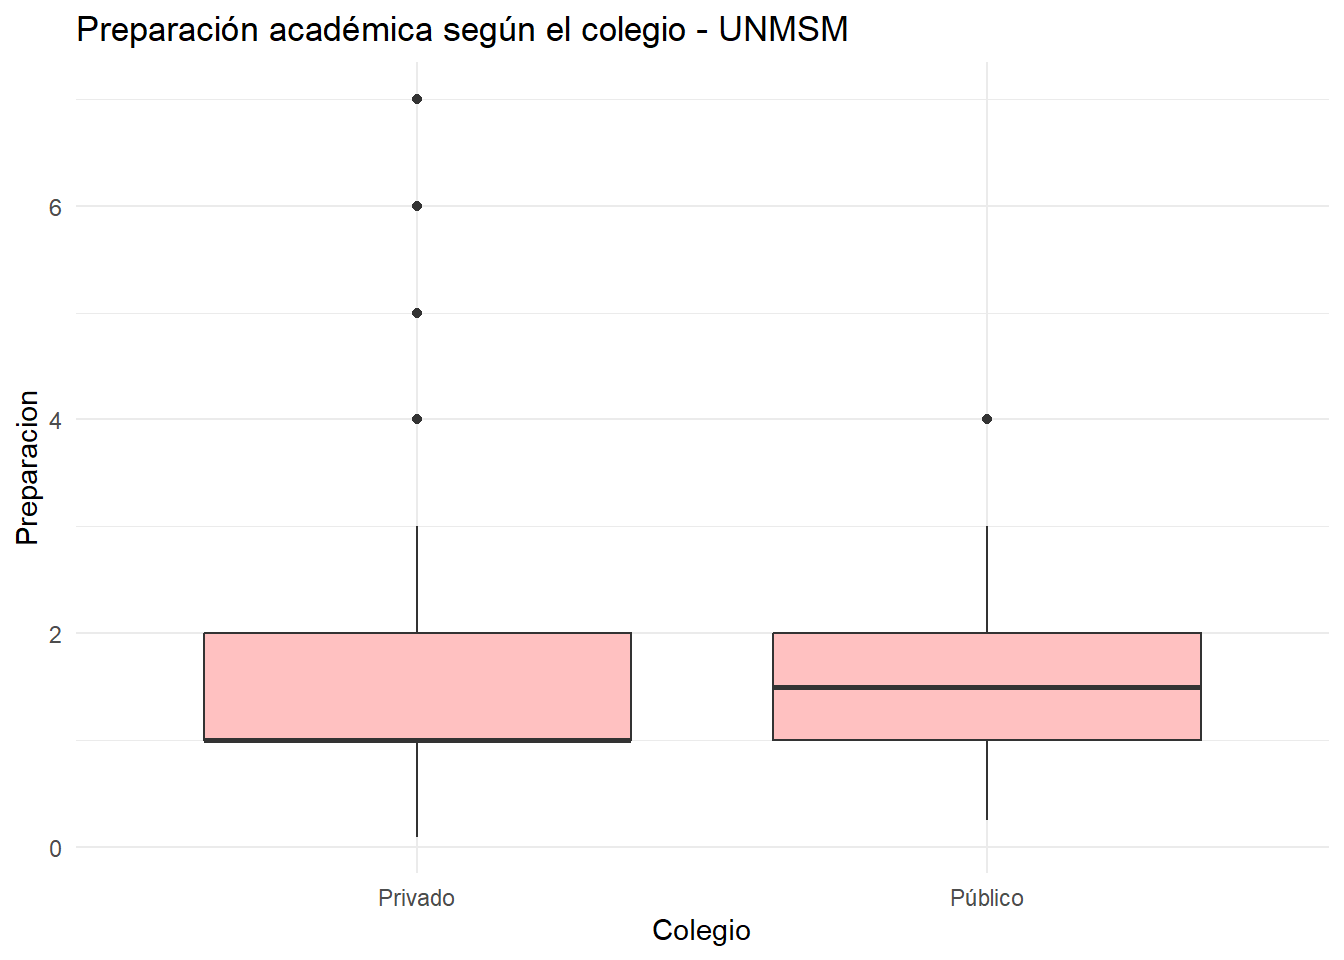
\includegraphics{S3_Informe_files/figure-latex/unnamed-chunk-16-1.pdf}

\begin{quote}
\hypertarget{explicaciuxf3n-2}{%
\subsection{\texorpdfstring{\textbf{\emph{EXPLICACIÓN:}}}{EXPLICACIÓN:}}\label{explicaciuxf3n-2}}
\end{quote}

Con este diagrama de barras se puede observar con mejor detenimiento
como es que se distribuye la variable ``Genero'', también podemos
observar que la menor variable de apariciones es ``Girls''. Por lo que
podemos concluir que los productos en MYNTRA son más aprovachos por
``Men'' y ``Woman'', además de que ``Girls'' no son clientes frecuentes
en temas de ``ropa de moda''.

\textbf{\emph{La media de precios de la empresa en USD:}}

\begin{Shaded}
\begin{Highlighting}[]
\FunctionTok{mean}\NormalTok{(dataMuestra}\SpecialCharTok{$}\NormalTok{PrecioUSD)}
\end{Highlighting}
\end{Shaded}

\begin{verbatim}
## [1] 20.80039
\end{verbatim}

La variable ``PrecioUSD'' tiene un promedio de 20.80039, pero esta
información no puede ser muy confiable ya que existen formas de dar
falsa información.

\textbf{\emph{La mediana de precios de la empresa en USD:}}

\begin{Shaded}
\begin{Highlighting}[]
\NormalTok{MedianaPrecio}\OtherTok{\textless{}{-}}\FunctionTok{median}\NormalTok{(dataMuestra}\SpecialCharTok{$}\NormalTok{PrecioUSD)}
\FunctionTok{print}\NormalTok{(MedianaPrecio)}
\end{Highlighting}
\end{Shaded}

\begin{verbatim}
## [1] 10.788
\end{verbatim}

Podemos observar que la tendencia central en la variable ``PrecioUSD''
es de 10.788 dolares.

\textbf{\emph{La moda de precios de la empresa en USD:}}

\begin{Shaded}
\begin{Highlighting}[]
\NormalTok{getmode }\OtherTok{\textless{}{-}} \ControlFlowTok{function}\NormalTok{(mod) \{}
\NormalTok{   uniqv }\OtherTok{\textless{}{-}} \FunctionTok{unique}\NormalTok{(mod)}
\NormalTok{   uniqv[}\FunctionTok{which.max}\NormalTok{(}\FunctionTok{tabulate}\NormalTok{(}\FunctionTok{match}\NormalTok{(mod, uniqv)))]}
\NormalTok{\}}
\NormalTok{mod }\OtherTok{\textless{}{-}}\NormalTok{ dataMuestra}\SpecialCharTok{$}\NormalTok{PrecioUSD}
\NormalTok{result }\OtherTok{\textless{}{-}} \FunctionTok{getmode}\NormalTok{(mod)}
\FunctionTok{print}\NormalTok{(result)}
\end{Highlighting}
\end{Shaded}

\begin{verbatim}
## [1] 8.388
\end{verbatim}

\begin{Shaded}
\begin{Highlighting}[]
\NormalTok{cantResult}\OtherTok{=}\FunctionTok{max}\NormalTok{(}\FunctionTok{table}\NormalTok{(mod))}
\FunctionTok{print}\NormalTok{(cantResult)}
\end{Highlighting}
\end{Shaded}

\begin{verbatim}
## [1] 63
\end{verbatim}

Podemos observar que el precio 8.388 dolares en la variable
``PrecioUSD'' es el que más se repite, siendo un total de 63 veces, por
lo que podemos concluir que el precio ideal para los productos es 8.388
dolares.

\begin{Shaded}
\begin{Highlighting}[]
\NormalTok{tablaPrecio}\OtherTok{\textless{}{-}}\FunctionTok{table}\NormalTok{(dataMuestra}\SpecialCharTok{$}\NormalTok{PrecioUSD)}
\NormalTok{tabla\_df }\OtherTok{\textless{}{-}} \FunctionTok{as.data.frame}\NormalTok{(tablaPrecio)}
\NormalTok{maxCantPrecio}\OtherTok{\textless{}{-}}\FunctionTok{max}\NormalTok{(tablaPrecio)}
\NormalTok{conteo}\OtherTok{\textless{}{-}}\NormalTok{tabla\_df}\SpecialCharTok{$}\NormalTok{Freq}
\CommentTok{\# Acceder al conteo}
\FunctionTok{plot}\NormalTok{(tabla\_df,}\FunctionTok{aes}\NormalTok{(}\AttributeTok{x=}\NormalTok{tabla\_df}\SpecialCharTok{$}\NormalTok{Var1,}\AttributeTok{y=}\NormalTok{tabla\_df}\SpecialCharTok{$}\NormalTok{Freq),}\AttributeTok{main=}\StringTok{"Rango de los precios"}\NormalTok{,}\AttributeTok{col=}\StringTok{"red"}\NormalTok{,}\AttributeTok{xlab=}\StringTok{"PreciosUSD"}\NormalTok{,}\AttributeTok{ylab=}\StringTok{"Cant. Apariciones"}\NormalTok{)}\SpecialCharTok{+}
\FunctionTok{geom\_line}\NormalTok{(}\AttributeTok{stat =} \StringTok{"identity"}\NormalTok{, }\AttributeTok{fill =} \FunctionTok{ifelse}\NormalTok{(conteo }\SpecialCharTok{==}\NormalTok{ maxCantPrecio, }\StringTok{"green"}\NormalTok{, }\StringTok{"blue"}\NormalTok{))}
\end{Highlighting}
\end{Shaded}

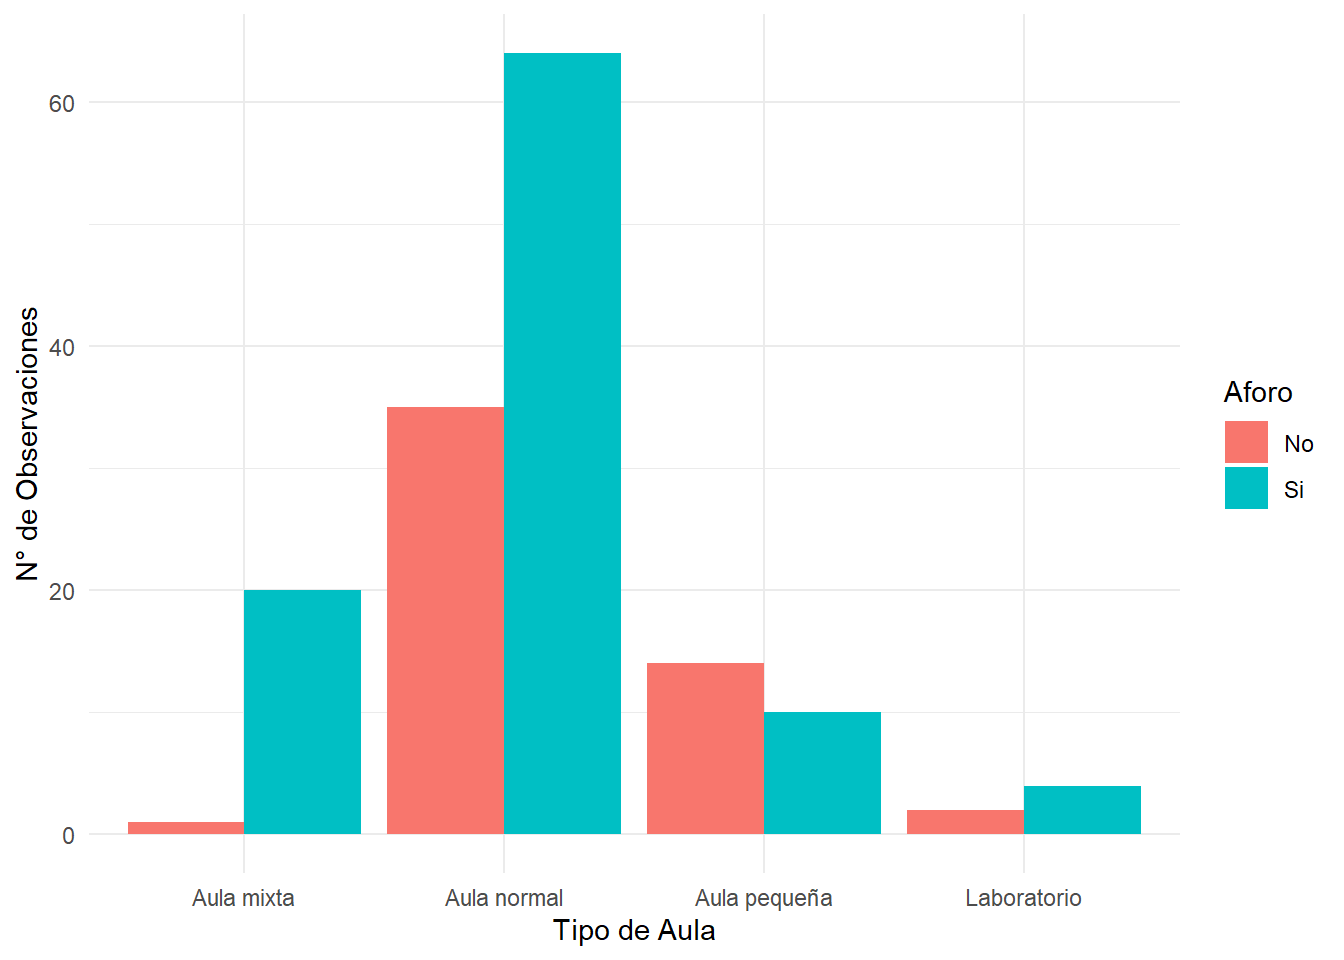
\includegraphics{S3_Informe_files/figure-latex/unnamed-chunk-20-1.pdf}

\begin{verbatim}
## NULL
\end{verbatim}

\begin{quote}
\hypertarget{explicaciuxf3n-3}{%
\subsection{\texorpdfstring{\textbf{EXPLICACIÓN:}}{EXPLICACIÓN:}}\label{explicaciuxf3n-3}}
\end{quote}

Podemos observar de mejor manera como se distribuyen los precios
respecto a sus apariciones, notando de que la cantidad de más
apariciones es del precio 8.38 con un total de 63 veces además de que
los precios menos 25 dolares son la preferencia de los clientes ya que
tienen una mayor cantidad de apariciones.

\textbf{\emph{El rango de los precios:}}

\begin{Shaded}
\begin{Highlighting}[]
\NormalTok{rango}\OtherTok{\textless{}{-}}\FunctionTok{range}\NormalTok{(dataMuestra}\SpecialCharTok{$}\NormalTok{PrecioUSD)}
\FunctionTok{print}\NormalTok{(}\StringTok{"inicia en:"}\NormalTok{)}
\end{Highlighting}
\end{Shaded}

\begin{verbatim}
## [1] "inicia en:"
\end{verbatim}

\begin{Shaded}
\begin{Highlighting}[]
\FunctionTok{print}\NormalTok{(rango[}\DecValTok{1}\NormalTok{])}
\end{Highlighting}
\end{Shaded}

\begin{verbatim}
## [1] 3.108
\end{verbatim}

\begin{Shaded}
\begin{Highlighting}[]
\FunctionTok{print}\NormalTok{(}\StringTok{"termina en:"}\NormalTok{)}
\end{Highlighting}
\end{Shaded}

\begin{verbatim}
## [1] "termina en:"
\end{verbatim}

\begin{Shaded}
\begin{Highlighting}[]
\FunctionTok{print}\NormalTok{(rango[}\DecValTok{2}\NormalTok{])}
\end{Highlighting}
\end{Shaded}

\begin{verbatim}
## [1] 373.2
\end{verbatim}

Los valores en la variable ``PrecioUSD'' están en un rango entre 3.108 y
373.2.

\begin{Shaded}
\begin{Highlighting}[]
\FunctionTok{hist}\NormalTok{(dataMuestra}\SpecialCharTok{$}\NormalTok{PrecioUSD,}\AttributeTok{col=}\FunctionTok{c}\NormalTok{(}\StringTok{"red"}\NormalTok{,}\StringTok{"blue"}\NormalTok{,}\StringTok{"yellow"}\NormalTok{,}\StringTok{"pink"}\NormalTok{),}\AttributeTok{main=}\StringTok{"Histograma de precios"}\NormalTok{,}\AttributeTok{xlab=}\StringTok{"Precios en USD"}\NormalTok{, }\AttributeTok{ylab=} \StringTok{"Cantidad"}\NormalTok{)}
\end{Highlighting}
\end{Shaded}

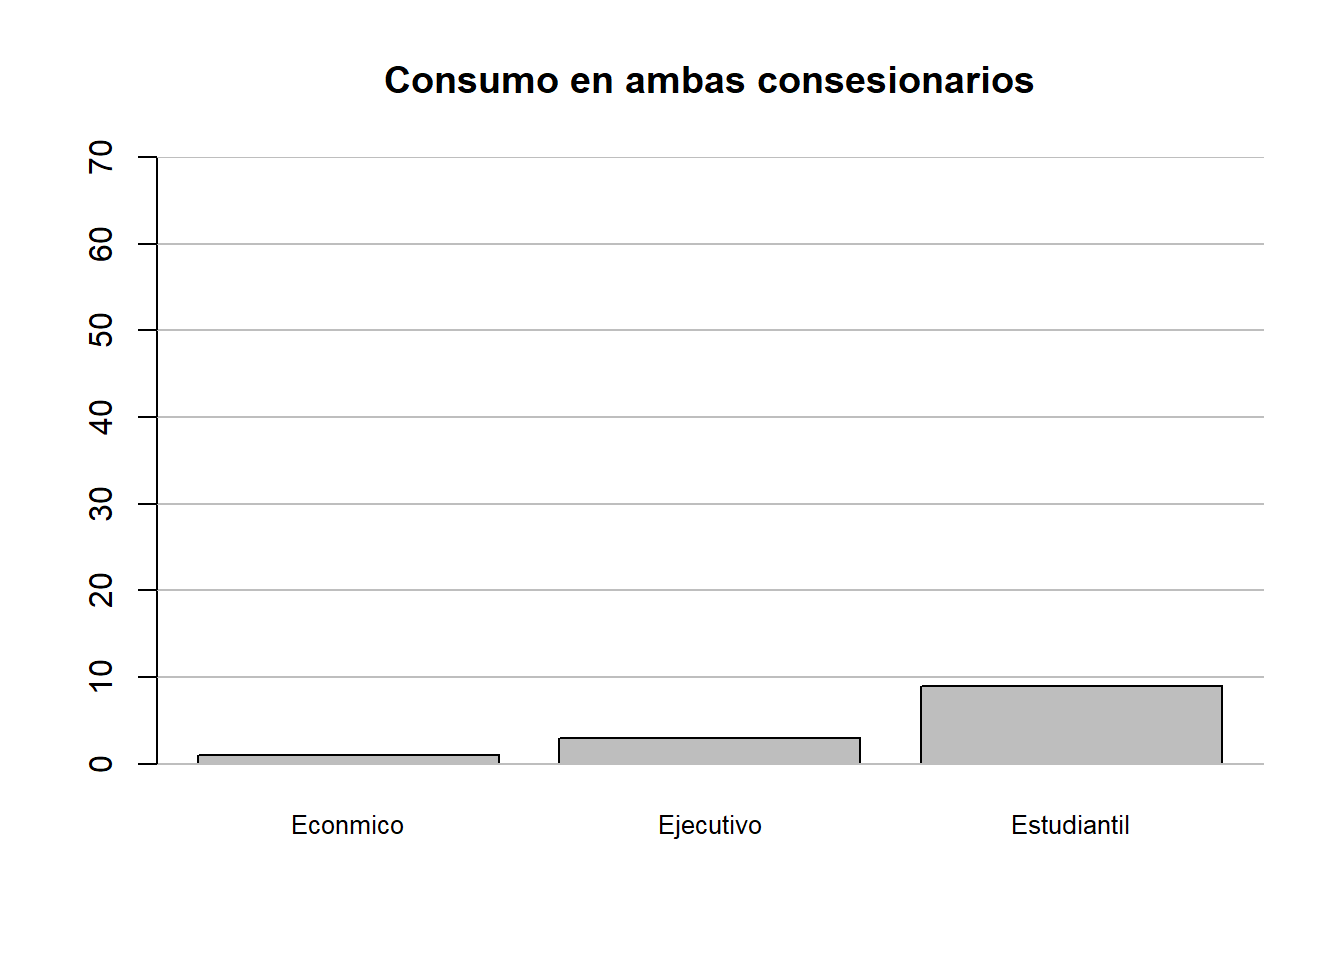
\includegraphics{S3_Informe_files/figure-latex/unnamed-chunk-22-1.pdf}

\begin{quote}
\hypertarget{explicaciuxf3n-4}{%
\subsection{\texorpdfstring{\textbf{\emph{EXPLICACIÓN:}}}{EXPLICACIÓN:}}\label{explicaciuxf3n-4}}
\end{quote}

Se puede observar de mejor manera como la mayor cantidad de apariciones
en los precios son inferiores a los 50 dolares aproximadamente, y que
los precios con menos apariciones son mayores a 100 dolares
proximadamente. Concluyendo que los clientes prefieren los productos más
baratos a 50 dolares.

\textbf{\emph{El rango intercuartil de precios:}}

\begin{Shaded}
\begin{Highlighting}[]
\NormalTok{Q1}\OtherTok{=}\FunctionTok{quantile}\NormalTok{(dataMuestra}\SpecialCharTok{$}\NormalTok{PrecioUSD,}\FloatTok{0.25}\NormalTok{)}\CommentTok{\#Q1}
\NormalTok{Q3}\OtherTok{=}\FunctionTok{quantile}\NormalTok{(dataMuestra}\SpecialCharTok{$}\NormalTok{PrecioUSD,}\FloatTok{0.75}\NormalTok{)}\CommentTok{\#Q1}
\NormalTok{Q3}\SpecialCharTok{{-}}\NormalTok{Q1}
\end{Highlighting}
\end{Shaded}

\begin{verbatim}
##   75% 
## 11.76
\end{verbatim}

\begin{Shaded}
\begin{Highlighting}[]
\CommentTok{\#segunda forma}
\FunctionTok{IQR}\NormalTok{(dataMuestra}\SpecialCharTok{$}\NormalTok{PrecioUSD)}
\end{Highlighting}
\end{Shaded}

\begin{verbatim}
## [1] 11.76
\end{verbatim}

\begin{Shaded}
\begin{Highlighting}[]
\FunctionTok{boxplot}\NormalTok{(dataMuestra}\SpecialCharTok{$}\NormalTok{PrecioUSD,}\AttributeTok{col=}\FunctionTok{c}\NormalTok{(}\StringTok{\textquotesingle{}yellow\textquotesingle{}}\NormalTok{),}\AttributeTok{horizontal =}\NormalTok{ T,}\AttributeTok{main=}\StringTok{"Rango de precios USD"}\NormalTok{)}
\end{Highlighting}
\end{Shaded}

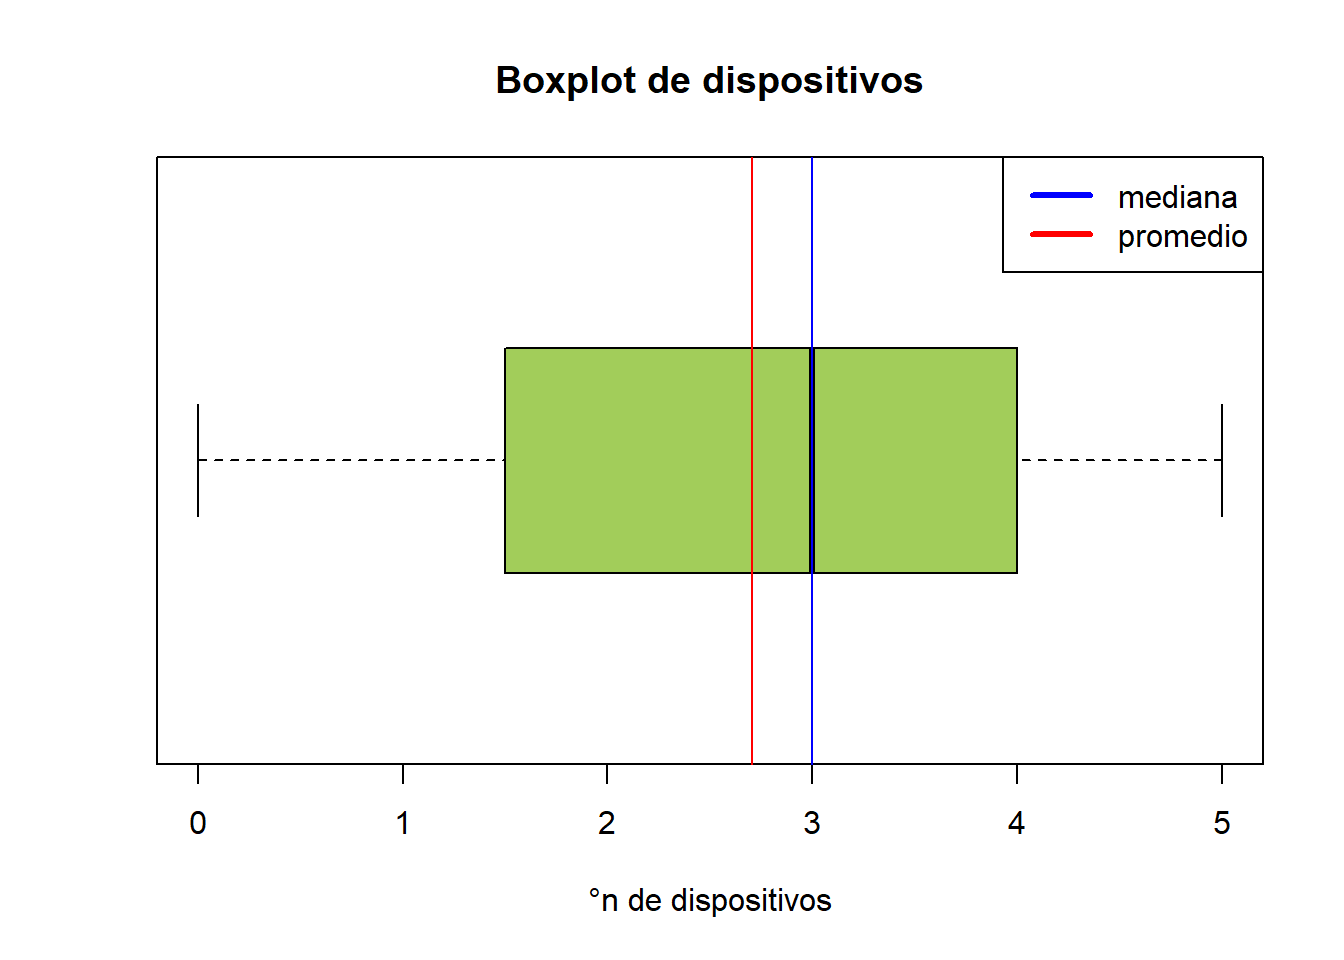
\includegraphics{S3_Informe_files/figure-latex/unnamed-chunk-23-1.pdf}

\begin{quote}
\hypertarget{explicaciuxf3n-5}{%
\subsection{\texorpdfstring{\textbf{\emph{EXPLICACIÓN:}}}{EXPLICACIÓN:}}\label{explicaciuxf3n-5}}
\end{quote}

En esta boxplot podemos observar que es sesgado a la derecha con valores
menores a 50 dolares, con n datos atípicos y que su su mediana está
alrededor de los 25 dolares aproximadamente. Podemos concluir que la
parte más corta es inferior a la mediana, y la media es mayor a la
mediana.

\textbf{\emph{La desviación estándar:}}

\begin{Shaded}
\begin{Highlighting}[]
\FunctionTok{sd}\NormalTok{(dataMuestra}\SpecialCharTok{$}\NormalTok{PrecioUSD)}\CommentTok{\#cuanto se dispersa el precio con respecto al promedio}
\end{Highlighting}
\end{Shaded}

\begin{verbatim}
## [1] 34.85258
\end{verbatim}

A partir de esta función la variación o dispersión en la que el precio
de los productos en USD difieren de la media.

\textbf{\emph{La varianza del precio:}}

\begin{Shaded}
\begin{Highlighting}[]
\FunctionTok{var}\NormalTok{(dataMuestra}\SpecialCharTok{$}\NormalTok{PrecioUSD)}
\end{Highlighting}
\end{Shaded}

\begin{verbatim}
## [1] 1214.702
\end{verbatim}

Podemos determinar que a mayor varianza del precio, mayor dispersión.

\textbf{\emph{El coeficiente de variación del precio:}}

\begin{Shaded}
\begin{Highlighting}[]
\NormalTok{coef\_var }\OtherTok{\textless{}{-}} \ControlFlowTok{function}\NormalTok{(cv, }\AttributeTok{na.rm =} \ConstantTok{TRUE}\NormalTok{) \{}
  \FunctionTok{sd}\NormalTok{(cv, }\AttributeTok{na.rm=}\NormalTok{na.rm) }\SpecialCharTok{/} \FunctionTok{mean}\NormalTok{(cv, }\AttributeTok{na.rm=}\NormalTok{na.rm)}
\NormalTok{\}}
\NormalTok{cv }\OtherTok{\textless{}{-}}\NormalTok{ dataMuestra}\SpecialCharTok{$}\NormalTok{PrecioUSD}
\FunctionTok{print}\NormalTok{(}\FunctionTok{coef\_var}\NormalTok{(cv))}
\end{Highlighting}
\end{Shaded}

\begin{verbatim}
## [1] 1.675573
\end{verbatim}

Es el análisis de las desviaciones del precio con respecto a la media y
al mismo tiempo las dispersiones que tienen los datos dispersos entre
sí.

\textbf{\emph{La moda de las imágenes}}

\begin{Shaded}
\begin{Highlighting}[]
\NormalTok{getmode }\OtherTok{\textless{}{-}} \ControlFlowTok{function}\NormalTok{(mod) \{}
\NormalTok{   uniqv }\OtherTok{\textless{}{-}} \FunctionTok{unique}\NormalTok{(mod)}
\NormalTok{   uniqv[}\FunctionTok{which.max}\NormalTok{(}\FunctionTok{tabulate}\NormalTok{(}\FunctionTok{match}\NormalTok{(mod, uniqv)))]}
\NormalTok{\}}

\NormalTok{mod }\OtherTok{\textless{}{-}}\NormalTok{ dataMuestra}\SpecialCharTok{$}\NormalTok{NumImagenes}
\NormalTok{result }\OtherTok{\textless{}{-}} \FunctionTok{getmode}\NormalTok{(mod)}
\FunctionTok{print}\NormalTok{(result)}
\end{Highlighting}
\end{Shaded}

\begin{verbatim}
## [1] 5
\end{verbatim}

\begin{Shaded}
\begin{Highlighting}[]
\FunctionTok{boxplot}\NormalTok{(dataMuestra}\SpecialCharTok{$}\NormalTok{NumImagenes,}\AttributeTok{horizontal =}\NormalTok{ T,}\AttributeTok{col=}\StringTok{"skyblue"}\NormalTok{,}\AttributeTok{main=}\StringTok{"Numero de Img"}\NormalTok{)}
\end{Highlighting}
\end{Shaded}

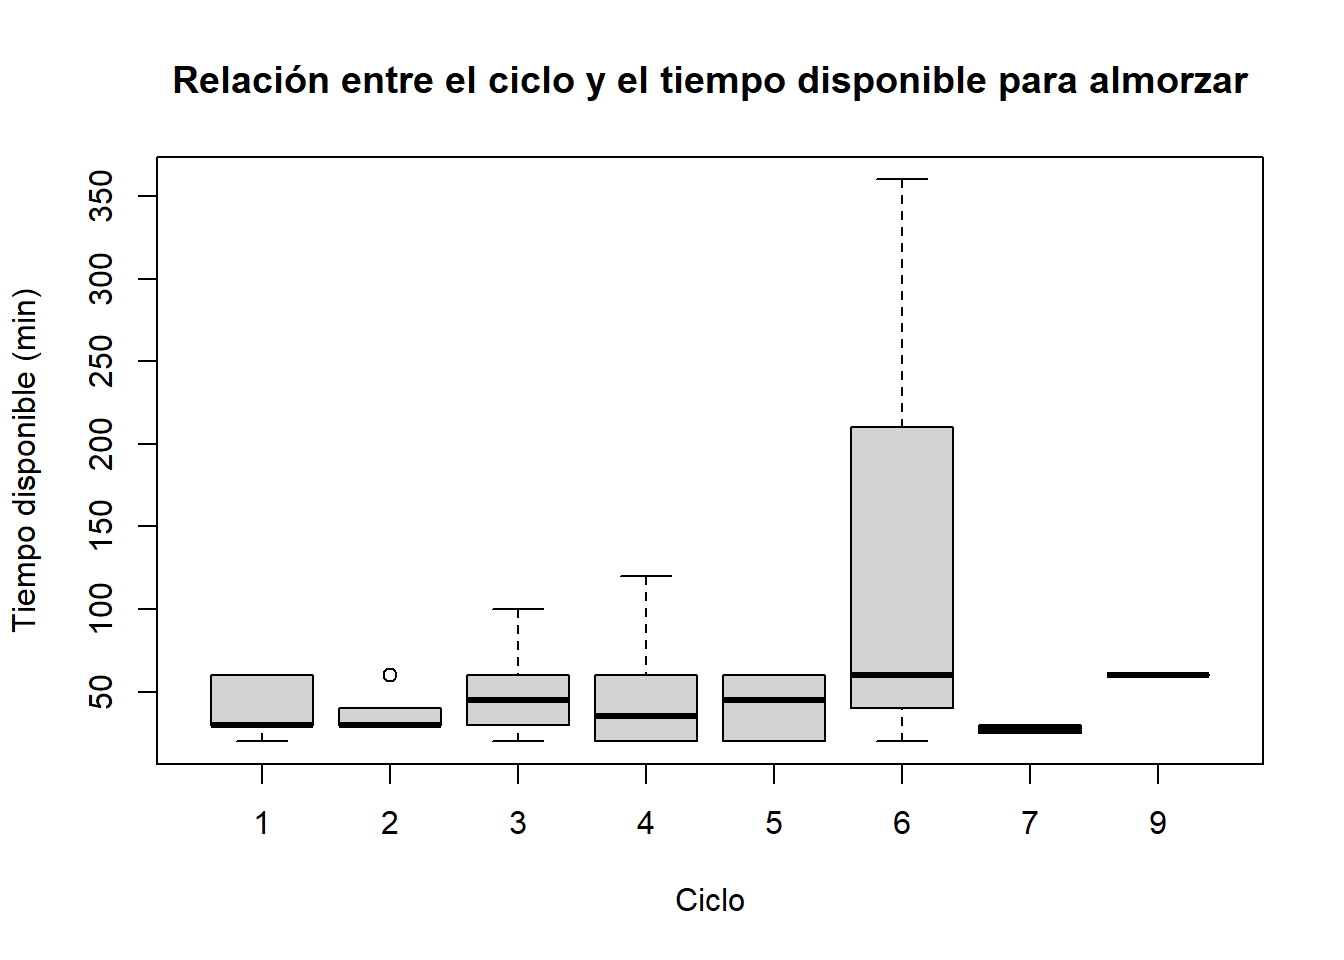
\includegraphics{S3_Informe_files/figure-latex/unnamed-chunk-27-1.pdf}

\begin{Shaded}
\begin{Highlighting}[]
\FunctionTok{print}\NormalTok{(}\StringTok{"Promedio:"}\NormalTok{)}
\end{Highlighting}
\end{Shaded}

\begin{verbatim}
## [1] "Promedio:"
\end{verbatim}

\begin{Shaded}
\begin{Highlighting}[]
\FunctionTok{mean}\NormalTok{(dataMuestra}\SpecialCharTok{$}\NormalTok{NumImagenes)}
\end{Highlighting}
\end{Shaded}

\begin{verbatim}
## [1] 4.607
\end{verbatim}

\begin{Shaded}
\begin{Highlighting}[]
\FunctionTok{print}\NormalTok{(}\StringTok{"Mediana:"}\NormalTok{)}
\end{Highlighting}
\end{Shaded}

\begin{verbatim}
## [1] "Mediana:"
\end{verbatim}

\begin{Shaded}
\begin{Highlighting}[]
\FunctionTok{median}\NormalTok{(dataMuestra}\SpecialCharTok{$}\NormalTok{NumImagenes)}
\end{Highlighting}
\end{Shaded}

\begin{verbatim}
## [1] 5
\end{verbatim}

\begin{quote}
\hypertarget{explicaciuxf3n-6}{%
\subsection{\texorpdfstring{\textbf{\emph{EXPLICACIÓN:}}}{EXPLICACIÓN:}}\label{explicaciuxf3n-6}}
\end{quote}

Podemos observar que tambien presenta datos atípicos, pero algo curioso
pasa en este boxplot, podemos ver que la mediana, media y la moda es
aproximadamente 5, es decir podemos concluir que la distribución es
simétrica.

\begin{Shaded}
\begin{Highlighting}[]
\NormalTok{tablaImagenes}\OtherTok{\textless{}{-}}\FunctionTok{table}\NormalTok{(mod)}
\FunctionTok{barplot}\NormalTok{(tablaImagenes,}\AttributeTok{col=}\FunctionTok{c}\NormalTok{(}\StringTok{\textquotesingle{}red\textquotesingle{}}\NormalTok{,}\StringTok{\textquotesingle{}blue\textquotesingle{}}\NormalTok{,}\StringTok{\textquotesingle{}pink\textquotesingle{}}\NormalTok{,}\StringTok{\textquotesingle{}yellow\textquotesingle{}}\NormalTok{,}\StringTok{\textquotesingle{}brown\textquotesingle{}}\NormalTok{,}\StringTok{\textquotesingle{}skyblue\textquotesingle{}}\NormalTok{,}\StringTok{\textquotesingle{}lightgreen\textquotesingle{}}\NormalTok{),}\AttributeTok{main=}\StringTok{"Diagra de barras de Num. Imagenes"}\NormalTok{)}
\end{Highlighting}
\end{Shaded}

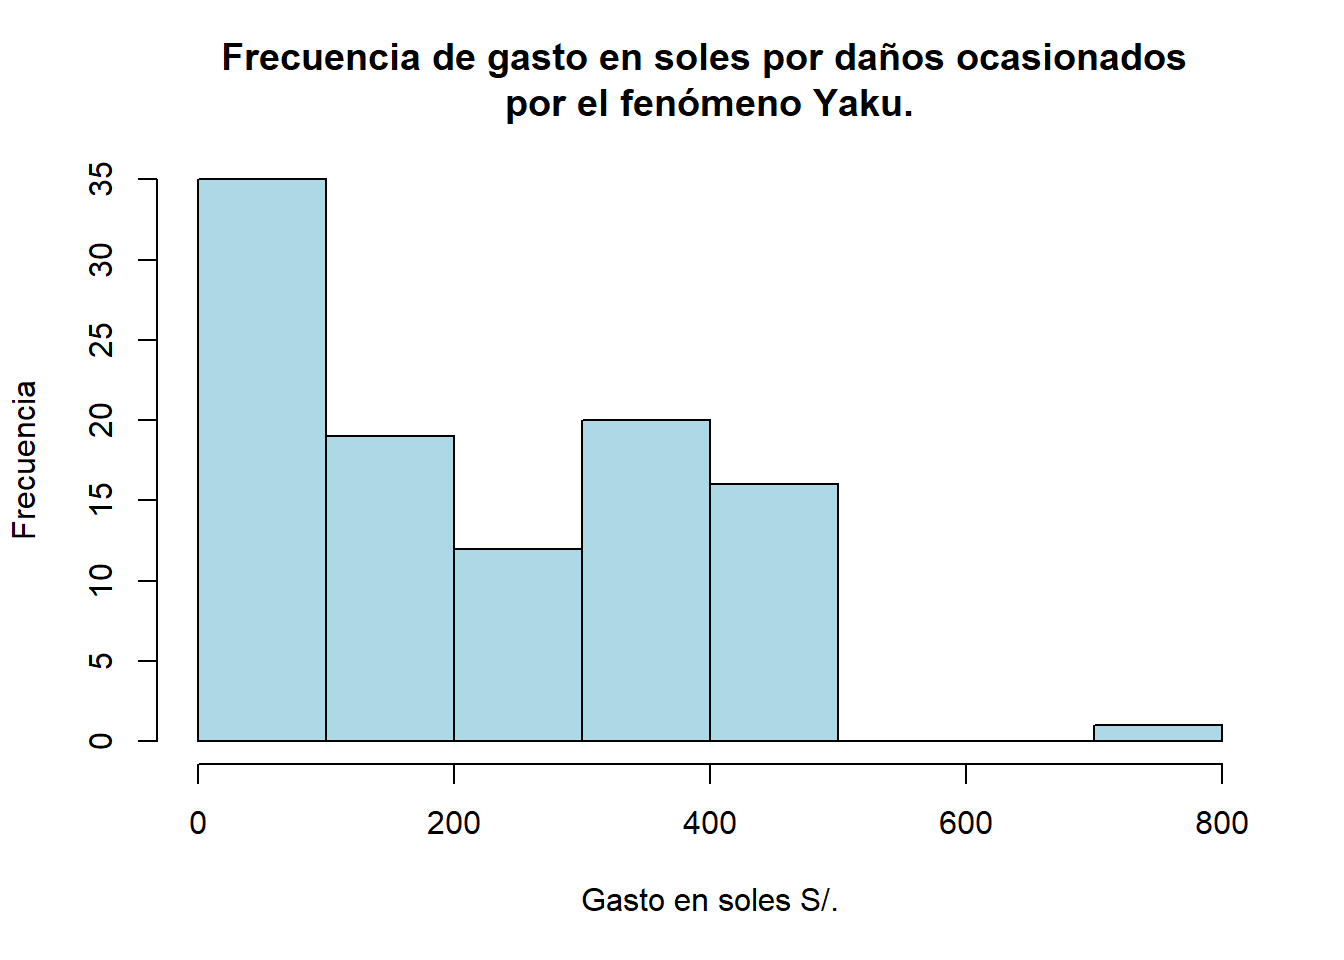
\includegraphics{S3_Informe_files/figure-latex/unnamed-chunk-28-1.pdf}
\textgreater{} \#\# \textbf{\emph{EXPLICACIÓN:}}

De una mejor manera podemos observar como es que las cantidades de los
precios es que se encuentran. Con ello podemos concluir que las empresas
con mayor éxito solo necesitan 5 imágenes para captar la atención del
cliente.

\textbf{\emph{Identificar el producto más caro:}}

\begin{Shaded}
\begin{Highlighting}[]
\FunctionTok{max}\NormalTok{(dataMuestra}\SpecialCharTok{$}\NormalTok{PrecioUSD)}
\end{Highlighting}
\end{Shaded}

\begin{verbatim}
## [1] 373.2
\end{verbatim}

\begin{Shaded}
\begin{Highlighting}[]
\NormalTok{productoCaro}\OtherTok{\textless{}{-}}\NormalTok{dataMuestra}\SpecialCharTok{\%\textgreater{}\%}
  \FunctionTok{filter}\NormalTok{(dataMuestra}\SpecialCharTok{$}\NormalTok{PrecioUSD}\SpecialCharTok{==}\FunctionTok{max}\NormalTok{(dataMuestra}\SpecialCharTok{$}\NormalTok{PrecioUSD))}
\NormalTok{productoCaro}
\end{Highlighting}
\end{Shaded}

\begin{verbatim}
## # A tibble: 2 x 8
##   ProductoId NombreProducto           MarcaProducto Genero PrecioUSD NumImagenes
##        <dbl> <chr>                    <chr>         <chr>      <dbl>       <dbl>
## 1   10017433 DKNY Unisex Purple Larg~ DKNY          Unisex      373.           7
## 2   10017461 DKNY Unisex Black & Gre~ DKNY          Unisex      373.           7
## # i 2 more variables: Descripción <chr>, ColorPrimario <chr>
\end{verbatim}

\begin{Shaded}
\begin{Highlighting}[]
\FunctionTok{unique}\NormalTok{(productoCaro}\SpecialCharTok{$}\NormalTok{MarcaProducto)}
\end{Highlighting}
\end{Shaded}

\begin{verbatim}
## [1] "DKNY"
\end{verbatim}

\begin{Shaded}
\begin{Highlighting}[]
\FunctionTok{unique}\NormalTok{(productoCaro}\SpecialCharTok{$}\NormalTok{Genero)}
\end{Highlighting}
\end{Shaded}

\begin{verbatim}
## [1] "Unisex"
\end{verbatim}

\begin{Shaded}
\begin{Highlighting}[]
\FunctionTok{unique}\NormalTok{(productoCaro}\SpecialCharTok{$}\NormalTok{ColorPrimario)}
\end{Highlighting}
\end{Shaded}

\begin{verbatim}
## [1] "Purple" "Black"
\end{verbatim}

El producto más caro es de la marca ``DKNY'' para los generos de
``Unisex'' con un precio de 373.2 dolares con los colores Purple y
Black.

\textbf{\emph{Identificar los colores más repetidos que llevan el
aumento de precio: }}

\begin{Shaded}
\begin{Highlighting}[]
\NormalTok{Modcolor}\OtherTok{\textless{}{-}}\FunctionTok{getmode}\NormalTok{(dataMuestra}\SpecialCharTok{$}\NormalTok{ColorPrimario)}
\FunctionTok{print}\NormalTok{(Modcolor)}
\end{Highlighting}
\end{Shaded}

\begin{verbatim}
## [1] "Blue"
\end{verbatim}

\begin{Shaded}
\begin{Highlighting}[]
\NormalTok{preguntaColor}\OtherTok{\textless{}{-}}\NormalTok{dataMuestra }\SpecialCharTok{\%\textgreater{}\%}
  \FunctionTok{filter}\NormalTok{(dataMuestra}\SpecialCharTok{$}\NormalTok{ColorPrimario}\SpecialCharTok{==}\NormalTok{Modcolor)}
\NormalTok{ModPrecioColor}\OtherTok{\textless{}{-}}\FunctionTok{getmode}\NormalTok{(preguntaColor}\SpecialCharTok{$}\NormalTok{PrecioUSD)}
\FunctionTok{print}\NormalTok{(ModPrecioColor)}
\end{Highlighting}
\end{Shaded}

\begin{verbatim}
## [1] 8.388
\end{verbatim}

\begin{Shaded}
\begin{Highlighting}[]
\NormalTok{cantResultColor}\OtherTok{\textless{}{-}}\FunctionTok{max}\NormalTok{(}\FunctionTok{table}\NormalTok{(preguntaColor}\SpecialCharTok{$}\NormalTok{PrecioUSD))}

\FunctionTok{barplot}\NormalTok{(}\FunctionTok{table}\NormalTok{(preguntaColor}\SpecialCharTok{$}\NormalTok{PrecioUSD), }\AttributeTok{col=} \FunctionTok{ifelse}\NormalTok{(}\FunctionTok{table}\NormalTok{(preguntaColor}\SpecialCharTok{$}\NormalTok{PrecioUSD)}\SpecialCharTok{==}\NormalTok{cantResultColor,}\StringTok{"red"}\NormalTok{,}\StringTok{"green"}\NormalTok{), }\AttributeTok{main=}\StringTok{"Diagrama de barras de los precios para los colores preferidos"}\NormalTok{)}
\end{Highlighting}
\end{Shaded}

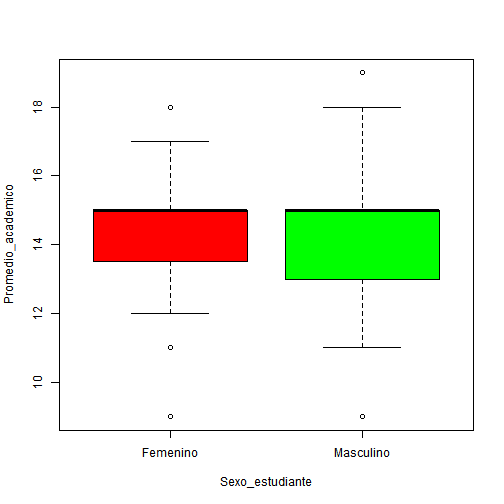
\includegraphics{S3_Informe_files/figure-latex/unnamed-chunk-30-1.pdf}

\begin{Shaded}
\begin{Highlighting}[]
\FunctionTok{range}\NormalTok{(preguntaColor}\SpecialCharTok{$}\NormalTok{PrecioUSD)}
\end{Highlighting}
\end{Shaded}

\begin{verbatim}
## [1]  3.192 67.188
\end{verbatim}

\begin{Shaded}
\begin{Highlighting}[]
\NormalTok{MasCaro}\OtherTok{\textless{}{-}}\NormalTok{preguntaColor}\SpecialCharTok{\%\textgreater{}\%}
  \FunctionTok{filter}\NormalTok{(preguntaColor}\SpecialCharTok{$}\NormalTok{PrecioUSD}\SpecialCharTok{==}\FunctionTok{max}\NormalTok{(preguntaColor}\SpecialCharTok{$}\NormalTok{PrecioUSD))}
\FunctionTok{print}\NormalTok{(MasCaro)}
\end{Highlighting}
\end{Shaded}

\begin{verbatim}
## # A tibble: 1 x 8
##   ProductoId NombreProducto           MarcaProducto Genero PrecioUSD NumImagenes
##        <dbl> <chr>                    <chr>         <chr>      <dbl>       <dbl>
## 1   10015921 Raymond Men Blue Self-D~ Raymond       Men         67.2           5
## # i 2 more variables: Descripción <chr>, ColorPrimario <chr>
\end{verbatim}

\begin{quote}
\hypertarget{explicaciuxf3n-7}{%
\subsection{\texorpdfstring{\textbf{\emph{EXPLICACIÓN:}}}{EXPLICACIÓN:}}\label{explicaciuxf3n-7}}
\end{quote}

Podemos observar que el color azul es el más preferido de las empresas,
también que su precio más repetido es de 8.388, y se encuentra en un
rango entre 3.192 y 67.188, además de que observamos de que el producto
más caro con un precio de 67.188, que es destinado a los hombre, de la
marca Raymond.

Con lo que podemos concluir que al alza de precio para los colores más
caros, depende de la ``Marca'' y para el género ``Cliente''.

\textbf{\emph{Cuáles son los precios más caros para los Varones:}}

\begin{Shaded}
\begin{Highlighting}[]
\FunctionTok{table}\NormalTok{(dataMuestra}\SpecialCharTok{$}\NormalTok{Genero) }
\end{Highlighting}
\end{Shaded}

\begin{verbatim}
## 
##   Boys  Girls    Men Unisex  Women 
##     63     43    373    148    373
\end{verbatim}

\begin{Shaded}
\begin{Highlighting}[]
\NormalTok{preguntaBoys}\OtherTok{\textless{}{-}}\NormalTok{ dataMuestra }\SpecialCharTok{\%\textgreater{}\%}
  \FunctionTok{filter}\NormalTok{(dataMuestra}\SpecialCharTok{$}\NormalTok{Genero}\SpecialCharTok{==}\StringTok{\textquotesingle{}Boys\textquotesingle{}}\NormalTok{)}

\NormalTok{MaxBoys}\OtherTok{=}\FunctionTok{max}\NormalTok{(preguntaBoys}\SpecialCharTok{$}\NormalTok{PrecioUSD)}
\FunctionTok{print}\NormalTok{(}\StringTok{"Marcas: "}\NormalTok{)}
\end{Highlighting}
\end{Shaded}

\begin{verbatim}
## [1] "Marcas: "
\end{verbatim}

\begin{Shaded}
\begin{Highlighting}[]
\FunctionTok{unique}\NormalTok{(preguntaBoys}\SpecialCharTok{$}\NormalTok{MarcaProducto)}
\end{Highlighting}
\end{Shaded}

\begin{verbatim}
## [1] "Gini and Jony"            "VASTRAMAY"               
## [3] "JBN Creation"             "U.S. Polo Assn. Kids"    
## [5] "Palm Tree"                "Aj DEZInES"              
## [7] "Marvel by Wear Your Mind" "Bubblegummers"
\end{verbatim}

\begin{Shaded}
\begin{Highlighting}[]
\FunctionTok{print}\NormalTok{(}\StringTok{\textquotesingle{}Precio maximo para Boys:\textquotesingle{}}\NormalTok{)}
\end{Highlighting}
\end{Shaded}

\begin{verbatim}
## [1] "Precio maximo para Boys:"
\end{verbatim}

\begin{Shaded}
\begin{Highlighting}[]
\FunctionTok{print}\NormalTok{(MaxBoys)}
\end{Highlighting}
\end{Shaded}

\begin{verbatim}
## [1] 20.388
\end{verbatim}

\begin{Shaded}
\begin{Highlighting}[]
\NormalTok{preguntaMen}\OtherTok{\textless{}{-}}\NormalTok{ dataMuestra }\SpecialCharTok{\%\textgreater{}\%}
  \FunctionTok{filter}\NormalTok{(dataMuestra}\SpecialCharTok{$}\NormalTok{Genero}\SpecialCharTok{==}\StringTok{\textquotesingle{}Men\textquotesingle{}}\NormalTok{)}
\NormalTok{MaxMens}\OtherTok{=}\FunctionTok{max}\NormalTok{(preguntaMen}\SpecialCharTok{$}\NormalTok{PrecioUSD)}
\FunctionTok{print}\NormalTok{(}\StringTok{"Marcas: "}\NormalTok{)}
\end{Highlighting}
\end{Shaded}

\begin{verbatim}
## [1] "Marcas: "
\end{verbatim}

\begin{Shaded}
\begin{Highlighting}[]
\FunctionTok{unique}\NormalTok{(preguntaMen}\SpecialCharTok{$}\NormalTok{MarcaProducto)}
\end{Highlighting}
\end{Shaded}

\begin{verbatim}
##  [1] "Raymond"                   "Parx"                     
##  [3] "SHOWOFF"                   "Police"                   
##  [5] "Being Human"               "YAK YAK"                  
##  [7] "HIGHLANDER"                "JEWEL JUNCTION"           
##  [9] "ID"                        "Difference of Opinion"    
## [11] "Michael Kors"              "Urban Dog"                
## [13] "Campus Sutra"              "FIDO DIDO"                
## [15] "Peter England"             "AIGNER"                   
## [17] "U.S. Polo Assn. Denim Co." "Sweet Dreams"             
## [19] "Qraa Men"                  "WITH"                     
## [21] "ColorPlus"                 "Arrow"                    
## [23] "DAVID BECKHAM"             "Carrera"                  
## [25] "HARBORNBAY"                "even"                     
## [27] "Crimsoune Club"            "Puma"                     
## [29] "Blackberrys"               "Park Avenue"              
## [31] "SIMON CARTER LONDON"       "Nautica"                  
## [33] "Bvlgari"                   "Hoopers"                  
## [35] "Peter England Casuals"     "GAS"                      
## [37] "VASTRAMAY"                 "Crew STREET"              
## [39] "Zippo"                     "aramis"                   
## [41] "HERE&NOW"                  "French Connection"        
## [43] "Next Look"                 "XYXX"                     
## [45] "Geox"
\end{verbatim}

\begin{Shaded}
\begin{Highlighting}[]
\FunctionTok{print}\NormalTok{(}\StringTok{\textquotesingle{}Precio maximo para Men:\textquotesingle{}}\NormalTok{)}
\end{Highlighting}
\end{Shaded}

\begin{verbatim}
## [1] "Precio maximo para Men:"
\end{verbatim}

\begin{Shaded}
\begin{Highlighting}[]
\FunctionTok{print}\NormalTok{(MaxMens)}
\end{Highlighting}
\end{Shaded}

\begin{verbatim}
## [1] 79.788
\end{verbatim}

\begin{Shaded}
\begin{Highlighting}[]
\NormalTok{TotalVarones}\OtherTok{=}\NormalTok{MaxBoys}\SpecialCharTok{+}\NormalTok{MaxMens}
\FunctionTok{print}\NormalTok{(}\StringTok{\textquotesingle{}Precio total:\textquotesingle{}}\NormalTok{)}
\end{Highlighting}
\end{Shaded}

\begin{verbatim}
## [1] "Precio total:"
\end{verbatim}

\begin{Shaded}
\begin{Highlighting}[]
\FunctionTok{print}\NormalTok{(TotalVarones)}
\end{Highlighting}
\end{Shaded}

\begin{verbatim}
## [1] 100.176
\end{verbatim}

\begin{quote}
\hypertarget{explicaciuxf3n-8}{%
\subsection{\texorpdfstring{\textbf{\emph{EXPLICACIÓN:}}}{EXPLICACIÓN:}}\label{explicaciuxf3n-8}}
\end{quote}

Podemos observar que los clientes más frecuentes son los Mens que los
Boys, como se dijo en la moda de ``Genero'', pero tambien podemos
obervar que los precios al menos uno de los más caros se encuentran en
los Mens, con un valor de 79.788 dolares. Dándonos un total de los
maximos precios para Mens y Boys con un precio de 100.176 dolares.

\textbf{\emph{Cuáles son los precios más caros para las Damas:}}

\begin{Shaded}
\begin{Highlighting}[]
\FunctionTok{table}\NormalTok{(dataMuestra}\SpecialCharTok{$}\NormalTok{Genero) }
\end{Highlighting}
\end{Shaded}

\begin{verbatim}
## 
##   Boys  Girls    Men Unisex  Women 
##     63     43    373    148    373
\end{verbatim}

\begin{Shaded}
\begin{Highlighting}[]
\NormalTok{preguntaGirls}\OtherTok{\textless{}{-}}\NormalTok{ dataMuestra }\SpecialCharTok{\%\textgreater{}\%}
  \FunctionTok{filter}\NormalTok{(dataMuestra}\SpecialCharTok{$}\NormalTok{Genero}\SpecialCharTok{==}\StringTok{\textquotesingle{}Girls\textquotesingle{}}\NormalTok{)}
\FunctionTok{print}\NormalTok{(}\StringTok{"Marcas: "}\NormalTok{)}
\end{Highlighting}
\end{Shaded}

\begin{verbatim}
## [1] "Marcas: "
\end{verbatim}

\begin{Shaded}
\begin{Highlighting}[]
\FunctionTok{unique}\NormalTok{(preguntaGirls}\SpecialCharTok{$}\NormalTok{MarcaProducto)}
\end{Highlighting}
\end{Shaded}

\begin{verbatim}
##  [1] "Gini and Jony"             "Stylo Bug"                
##  [3] "Palm Tree"                 "Playdate"                 
##  [5] "berrytree"                 "United Colors of Benetton"
##  [7] "Bubblegummers"             "Pink Cow"                 
##  [9] "Daffodils"                 "Bitiya by Bhama"
\end{verbatim}

\begin{Shaded}
\begin{Highlighting}[]
\NormalTok{MaxGirls}\OtherTok{=}\FunctionTok{max}\NormalTok{(preguntaGirls}\SpecialCharTok{$}\NormalTok{PrecioUSD)}
\FunctionTok{print}\NormalTok{(}\StringTok{\textquotesingle{}Precio maximo para Girls:\textquotesingle{}}\NormalTok{)}
\end{Highlighting}
\end{Shaded}

\begin{verbatim}
## [1] "Precio maximo para Girls:"
\end{verbatim}

\begin{Shaded}
\begin{Highlighting}[]
\FunctionTok{print}\NormalTok{(MaxGirls)}
\end{Highlighting}
\end{Shaded}

\begin{verbatim}
## [1] 45.6
\end{verbatim}

\begin{Shaded}
\begin{Highlighting}[]
\NormalTok{preguntaWomen}\OtherTok{\textless{}{-}}\NormalTok{ dataMuestra }\SpecialCharTok{\%\textgreater{}\%}
  \FunctionTok{filter}\NormalTok{(dataMuestra}\SpecialCharTok{$}\NormalTok{Genero}\SpecialCharTok{==}\StringTok{\textquotesingle{}Women\textquotesingle{}}\NormalTok{)}
\FunctionTok{print}\NormalTok{(}\StringTok{"Marcas: "}\NormalTok{)}
\end{Highlighting}
\end{Shaded}

\begin{verbatim}
## [1] "Marcas: "
\end{verbatim}

\begin{Shaded}
\begin{Highlighting}[]
\FunctionTok{unique}\NormalTok{(preguntaWomen}\SpecialCharTok{$}\NormalTok{MarcaProducto)}
\end{Highlighting}
\end{Shaded}

\begin{verbatim}
##  [1] "EthnoVogue"              "SPYKAR"                 
##  [3] "Kenneth Cole"            "Vishudh"                
##  [5] "PARFAIT"                 "Michael Kors"           
##  [7] "Sera"                    "AccessHer"              
##  [9] "Alcis"                   "Tokyo Talkies"          
## [11] "ANNA SUI"                "her by invictus"        
## [13] "Soie"                    "Lara Karen"             
## [15] "ahilya"                  "BuckleUp"               
## [17] "Lady Lyka"               "Park Avenue"            
## [19] "Roadster"                "Kazo"                   
## [21] "Bvlgari"                 "GAS"                    
## [23] "ZUSH"                    "DressBerry"             
## [25] "Lakme"                   "Allen Solly Woman"      
## [27] "MANGO"                   "Ishin"                  
## [29] "Shoe Couture"            "Keds"                   
## [31] "Rozia"                   "HARBORNBAY"             
## [33] "Monte Carlo"             "ether"                  
## [35] "Russell Athletic"        "MIMOSA"                 
## [37] "Rocia"                   "Annabelle by Pantaloons"
## [39] "DKNY"                    "Beli"                   
## [41] "Jn Joy"                  "THE SILHOUETTE STORE"   
## [43] "Xpose"                   "MBE"                    
## [45] "Mast & Harbour"          "JC Collection"          
## [47] "GUESS"                   "StyleStone"             
## [49] "SASSAFRAS"               "Kook N Keech Disney"    
## [51] "Honey by Pantaloons"     "Police"                 
## [53] "DOROTHY PERKINS"         "Bhama Couture"          
## [55] "Puma"                    "C9 AIRWEAR"             
## [57] "Oxolloxo"                "Crocs"                  
## [59] "Carlton London"          "shaze"                  
## [61] "Tulsattva"               "HERE&NOW"
\end{verbatim}

\begin{Shaded}
\begin{Highlighting}[]
\NormalTok{MaxWomen}\OtherTok{=}\FunctionTok{max}\NormalTok{(preguntaWomen}\SpecialCharTok{$}\NormalTok{PrecioUSD)}
\FunctionTok{print}\NormalTok{(}\StringTok{\textquotesingle{}Precio maximo para Women: \textquotesingle{}}\NormalTok{)}
\end{Highlighting}
\end{Shaded}

\begin{verbatim}
## [1] "Precio maximo para Women: "
\end{verbatim}

\begin{Shaded}
\begin{Highlighting}[]
\FunctionTok{print}\NormalTok{(MaxWomen)}
\end{Highlighting}
\end{Shaded}

\begin{verbatim}
## [1] 133.644
\end{verbatim}

\begin{Shaded}
\begin{Highlighting}[]
\NormalTok{TotalDamas}\OtherTok{=}\NormalTok{MaxGirls}\SpecialCharTok{+}\NormalTok{MaxWomen}
\FunctionTok{print}\NormalTok{(}\StringTok{\textquotesingle{}Precio total: \textquotesingle{}}\NormalTok{)}
\end{Highlighting}
\end{Shaded}

\begin{verbatim}
## [1] "Precio total: "
\end{verbatim}

\begin{Shaded}
\begin{Highlighting}[]
\FunctionTok{print}\NormalTok{(TotalDamas)}
\end{Highlighting}
\end{Shaded}

\begin{verbatim}
## [1] 179.244
\end{verbatim}

\begin{quote}
\hypertarget{explicaciuxf3n-9}{%
\subsection{\texorpdfstring{\textbf{\emph{EXPLICACIÓN:}}}{EXPLICACIÓN:}}\label{explicaciuxf3n-9}}
\end{quote}

Podemos observar que los clientes más frecuentes son las Women que las
Girls, como se dijo en la moda de ``Genero'', pero también podemos
obervar que los precios al menos uno de los más caros se encuentran en
las Women, con un valor de 133.644 dolares. Dándonos un total de los
maximos precios para Women y Girls con un precio de 179.244 dolares.

\begin{Shaded}
\begin{Highlighting}[]
\ControlFlowTok{if}\NormalTok{ (TotalDamas}\SpecialCharTok{\textgreater{}}\NormalTok{TotalVarones)\{}
  \FunctionTok{print}\NormalTok{(}\StringTok{"Las Damas tienen precio más caro con una diferencia de "}\NormalTok{)}
  \FunctionTok{print}\NormalTok{(TotalDamas}\SpecialCharTok{{-}}\NormalTok{TotalVarones)}
  \FunctionTok{print}\NormalTok{(}\StringTok{"Datos de la compra"}\NormalTok{)}
\NormalTok{  tablaResult}\OtherTok{\textless{}{-}}\NormalTok{preguntaWomen }\SpecialCharTok{\%\textgreater{}\%}
    \FunctionTok{filter}\NormalTok{(preguntaWomen}\SpecialCharTok{$}\NormalTok{PrecioUSD}\SpecialCharTok{==}\NormalTok{MaxWomen)}
\NormalTok{  tablaResult}
\NormalTok{\}}\ControlFlowTok{else}\NormalTok{\{}
  \FunctionTok{print}\NormalTok{(}\StringTok{"Los Varones tienen precio más caro con una diferencia de "}\NormalTok{)}
  \FunctionTok{print}\NormalTok{(TotalVarones}\SpecialCharTok{{-}}\NormalTok{TotalDamas)}
\NormalTok{\}}
\end{Highlighting}
\end{Shaded}

\begin{verbatim}
## [1] "Las Damas tienen precio más caro con una diferencia de "
## [1] 79.068
## [1] "Datos de la compra"
\end{verbatim}

\begin{verbatim}
## # A tibble: 1 x 8
##   ProductoId NombreProducto           MarcaProducto Genero PrecioUSD NumImagenes
##        <dbl> <chr>                    <chr>         <chr>      <dbl>       <dbl>
## 1    1000743 ahilya Gold-Plated Ster~ ahilya        Women       134.           3
## # i 2 more variables: Descripción <chr>, ColorPrimario <chr>
\end{verbatim}

Podemos concluir que las damas han comprado los productos más caros y
que son de la marca ``ahilya'', llamado ``ahilya Gold-Plated Sterling
Silver Jhumka Earrings'' y que es de color ``Gold''.

\textbf{\emph{El rango de los precios según el genero de la ropa:}}

\begin{Shaded}
\begin{Highlighting}[]
\FunctionTok{ggplot}\NormalTok{(}\AttributeTok{data =}\NormalTok{ dataMuestra, }\FunctionTok{aes}\NormalTok{(}\AttributeTok{x =}\NormalTok{ dataMuestra}\SpecialCharTok{$}\NormalTok{Genero, }\AttributeTok{y =}\NormalTok{ dataMuestra}\SpecialCharTok{$}\NormalTok{PrecioUSD, }\AttributeTok{fill =}\NormalTok{ dataMuestra}\SpecialCharTok{$}\NormalTok{Genero)) }\SpecialCharTok{+}
  \FunctionTok{geom\_boxplot}\NormalTok{() }\SpecialCharTok{+}
  \FunctionTok{labs}\NormalTok{(}\AttributeTok{title =} \StringTok{"Relación entre el Precio y el Género de la Ropa"}\NormalTok{,}
       \AttributeTok{x =} \StringTok{"Género"}\NormalTok{,}
       \AttributeTok{y =} \StringTok{"Precio"}\NormalTok{,}
       \AttributeTok{fill =} \StringTok{"Género"}\NormalTok{) }\SpecialCharTok{+}
  \FunctionTok{theme\_minimal}\NormalTok{()}
\end{Highlighting}
\end{Shaded}

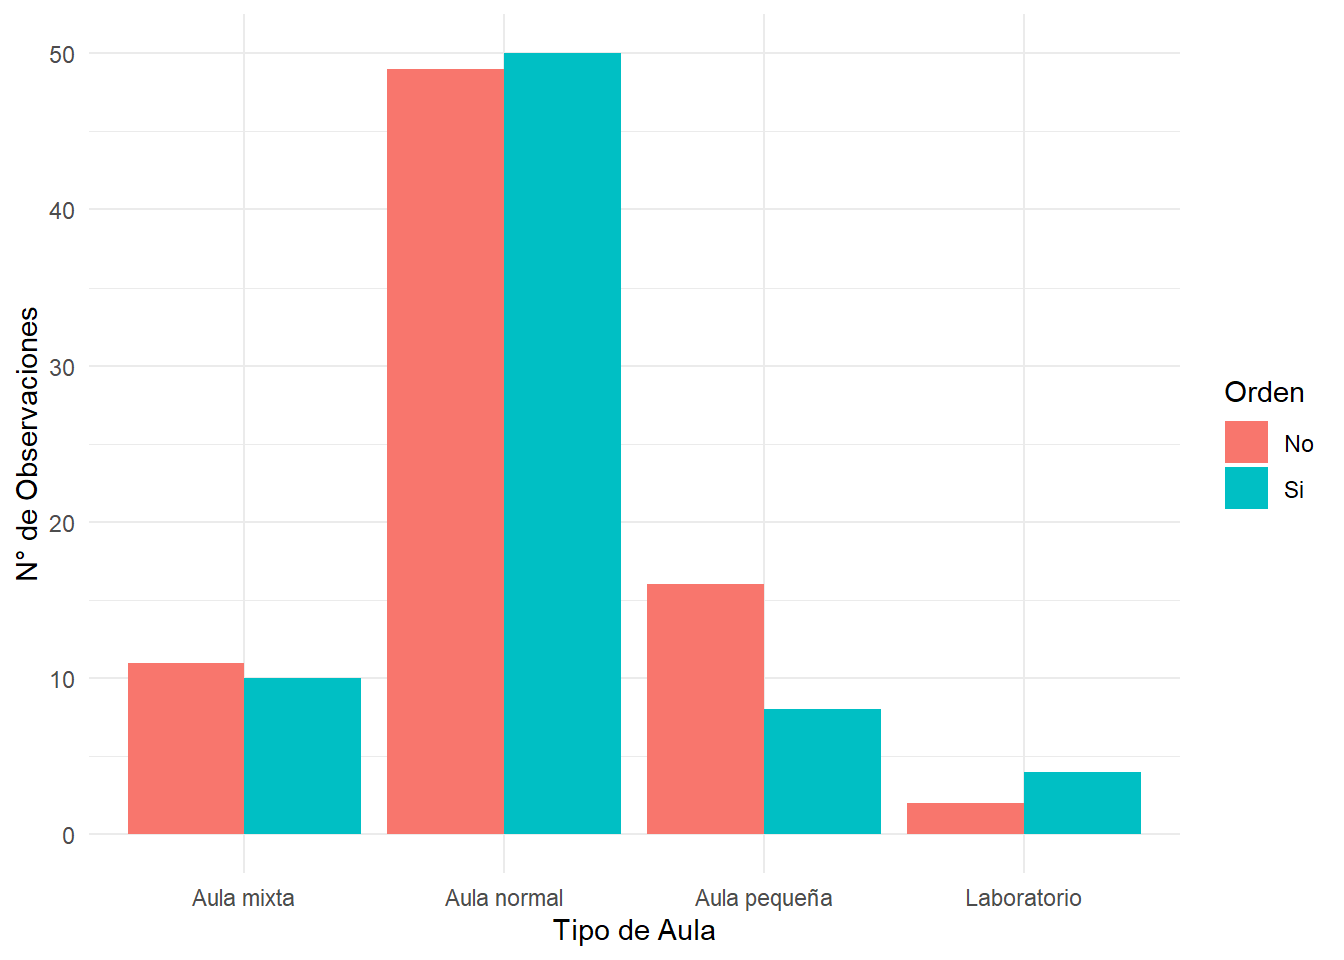
\includegraphics{S3_Informe_files/figure-latex/unnamed-chunk-34-1.pdf}

\begin{quote}
\hypertarget{explicaciuxf3n-10}{%
\subsection{\texorpdfstring{\textbf{\emph{EXPLICACIÓN:}}}{EXPLICACIÓN:}}\label{explicaciuxf3n-10}}
\end{quote}

Podemos apreciar que este gráfico nos da una relación entre el precio de
la ropa y el género al que va destinado, por lo que, podemos concluir
que la ropa unisex es de las mas costosas, superando los 300 dolares,
seguido por la ropa para mujeres y finalmete la ropa para hombres.
Además, la ropa para niños es la más económica, con un precio por debajo
de los 50 dolares.

\textbf{\emph{La cantidad de ropa Unisex que saca cada marca}}

\begin{Shaded}
\begin{Highlighting}[]
\NormalTok{dataHombres }\OtherTok{\textless{}{-}}\NormalTok{ dataMuestra }\SpecialCharTok{\%\textgreater{}\%} \FunctionTok{filter}\NormalTok{(Genero }\SpecialCharTok{==} \StringTok{"Unisex"}\NormalTok{)}
\FunctionTok{ggplot}\NormalTok{(}\AttributeTok{data =}\NormalTok{ dataHombres, }\FunctionTok{aes}\NormalTok{(}\AttributeTok{x =}\NormalTok{ dataHombres}\SpecialCharTok{$}\NormalTok{MarcaProducto, }\AttributeTok{fill =}\NormalTok{ dataHombres}\SpecialCharTok{$}\NormalTok{Genero)) }\SpecialCharTok{+}
  \FunctionTok{geom\_bar}\NormalTok{(}\AttributeTok{position=}\StringTok{"dodge"}\NormalTok{) }\SpecialCharTok{+}
  \FunctionTok{labs}\NormalTok{(}\AttributeTok{title =} \StringTok{"Relación entre la Marca y el Género de la Ropa"}\NormalTok{,}
       \AttributeTok{x =} \StringTok{"Marca"}\NormalTok{,}
       \AttributeTok{y =} \StringTok{"Conteo"}\NormalTok{,}
       \AttributeTok{fill =} \StringTok{"Género"}\NormalTok{) }\SpecialCharTok{+}
  \FunctionTok{theme\_minimal}\NormalTok{() }\SpecialCharTok{+}
  \FunctionTok{theme}\NormalTok{(}\AttributeTok{axis.text.x =} \FunctionTok{element\_text}\NormalTok{(}\AttributeTok{angle =} \DecValTok{90}\NormalTok{)) }
\end{Highlighting}
\end{Shaded}

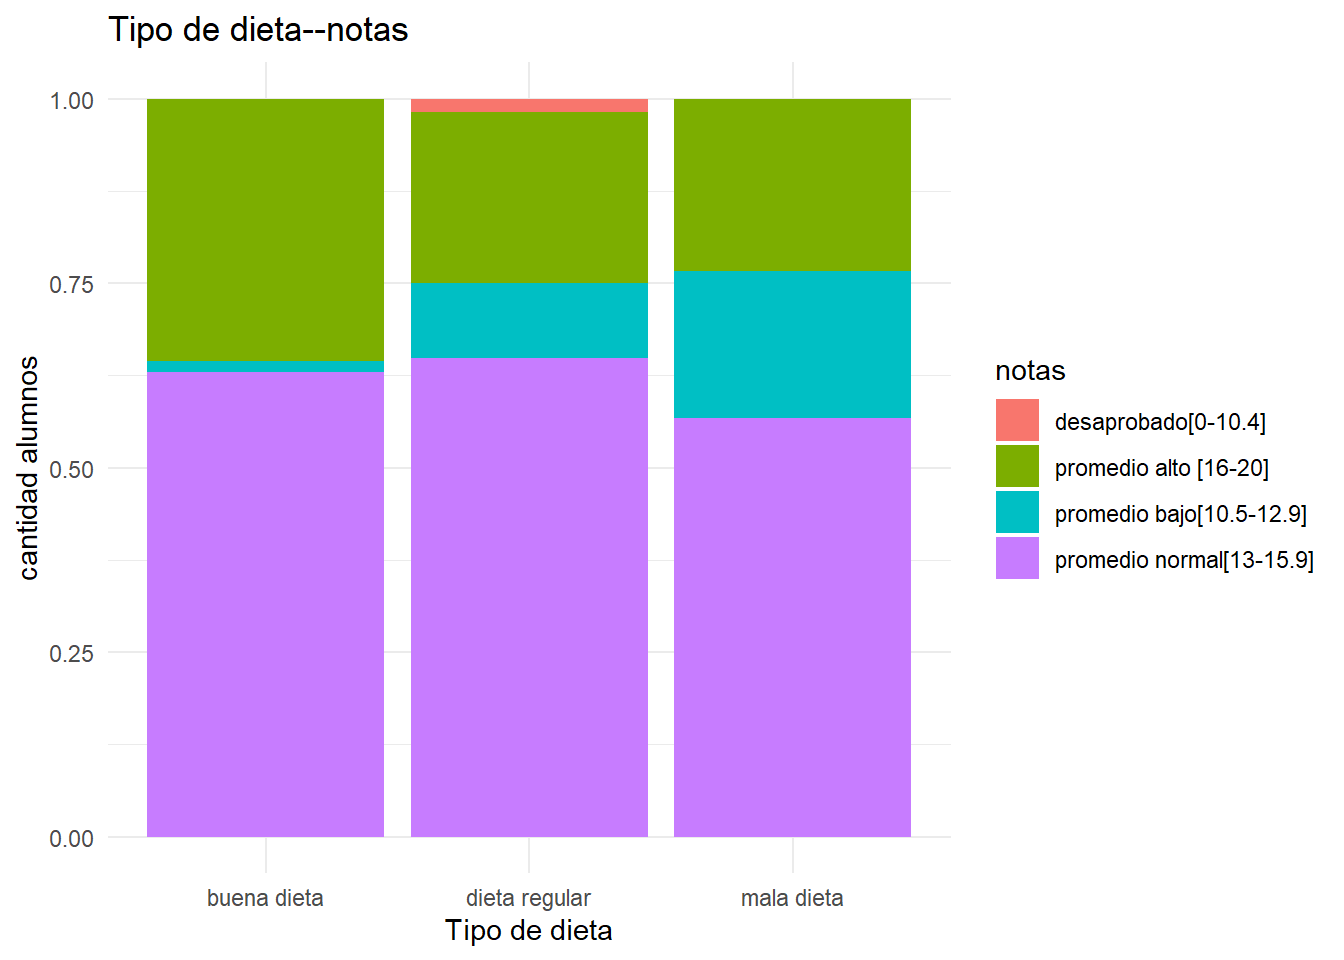
\includegraphics{S3_Informe_files/figure-latex/unnamed-chunk-35-1.pdf}

\begin{quote}
\hypertarget{explicaciuxf3n-11}{%
\subsection{\texorpdfstring{\textbf{\emph{EXPLICACIÓN:}}}{EXPLICACIÓN:}}\label{explicaciuxf3n-11}}
\end{quote}

Podemos apreciar, mediante un gráfico de barras que cada marca tienen
una preferencia en cuanto al genero de ropa Unisex en variación a los
demás géneros. De esta forma, se puede visualizar rápidamente que marcas
en el conjunto de datos dataMuestra producen una mayor cantidad de ropa
unisex.

\begin{quote}
\hypertarget{conclusiones}{%
\section{\texorpdfstring{\textbf{Conclusiones}}{Conclusiones}}\label{conclusiones}}
\end{quote}

\begin{enumerate}
\def\labelenumi{\arabic{enumi}.}
\item
  El producto preferido de los clientes es \textbf{``Parx Men Blue Slim
  Fit Checked Casual Shirt''}, mayormente comprado por hombres, con el
  color azul y sus precios rondan entre 8.148 y 11.268 dolares.
\item
  La marca preferida de los clientes es \textbf{``Parx''}, mayormente
  comprada por hombres, con colores muy variados pero con una
  preferencia del azul y sus precios rondan entre 4.188 y 11.748
  dolares.
\item
  Nuestros mayores clientes son \emph{Men} y \emph{Women} (hombres y
  mujeres), luego el género Unisex, continuando con Boys y el cliente
  menos común Girls.
\item
  Nuestros precios están en un rango entre \textbf{\emph{3.108 y 373.2
  dolares}}, el precio con el que los clientes prefieren comprar es de
  8.388 dolares, además de que también en el gráfico de puntos, podemos
  observar que los \textbf{precios menores a 50 también son más
  frecuentes} entre los clientes por sus cantidades de apariciones.
\item
  Como hemos observado en las conclusiones 1 y 2 el color azul es el que
  mayormente aparece, con un rango de precios entre \textbf{3.192 y
  67.188 dolares}, y que el alza de precio por el color se debe ala
  Marca y al género del cliente.
\item
  Analizando el precio entre los géneros, no hemos tomado en cuenta el
  género ``Unisex'' por que entraría en los dos casos y se terminaran
  restando, luego analizamos a todo el género \textbf{``Masculino'' (Men
  y Boys)} y a todo el género \textbf{``Femenino'' (Women y Girls)},
  luego los sumamos todos sus precios para luego restar esos dos
  géneros, entonces podemos ver que el género ``Femenino'' es el que
  tiene el precio más caro (133.644 dólares) de \textbf{\emph{la marca
  ``ahilya'' con el producto ``ahilya Gold-Plated Sterling Silver Jhumka
  Earrings'' de color dorado.}}
\end{enumerate}

\end{document}
